\documentclass{article}
\usepackage{amsmath,amssymb,amsthm,kotex,mdframed,paralist,chngcntr}
\usepackage{subcaption}

\newcounter{num}
%\newcommand{\defi}[1]
%{\bigskip\noindent\refstepcounter{num}\textbf{정의 \arabic{num}) #1}\par}
%\newcommand{\theo}[1]
%{\bigskip\noindent\refstepcounter{num}\textbf{정리 \arabic{num}) #1}\par}
%\newcommand{\exam}[1]
%{\bigskip\noindent\refstepcounter{num}\textbf{예시 \arabic{num}) #1}\par}
%\newcommand{\prob}[1]
%{\bigskip\noindent\refstepcounter{num}\textbf{문제 \arabic{num}) #1}\par}
\newcommand{\howo}[1]
{\bigskip\noindent\refstepcounter{num}\textbf{숙제 \arabic{num}) #1}\par\bigskip}


\renewcommand{\proofname}{증명)}
\counterwithout{subsection}{section}


%%%
\begin{document}

\title{영석 : 11 숙제(\(\sim\)2015. 6. 27. 토요일)}
\author{}
\date{\today}
\maketitle
%\tableofcontents
\newpage

%
\howo{}
다음 부등식의 영역을 좌표 평면 위에 나타내어라.
\[y>2x+1\]

\begin{figure}[h!]
        \centering
        \begin{subfigure}[b]{0.18\textwidth}
                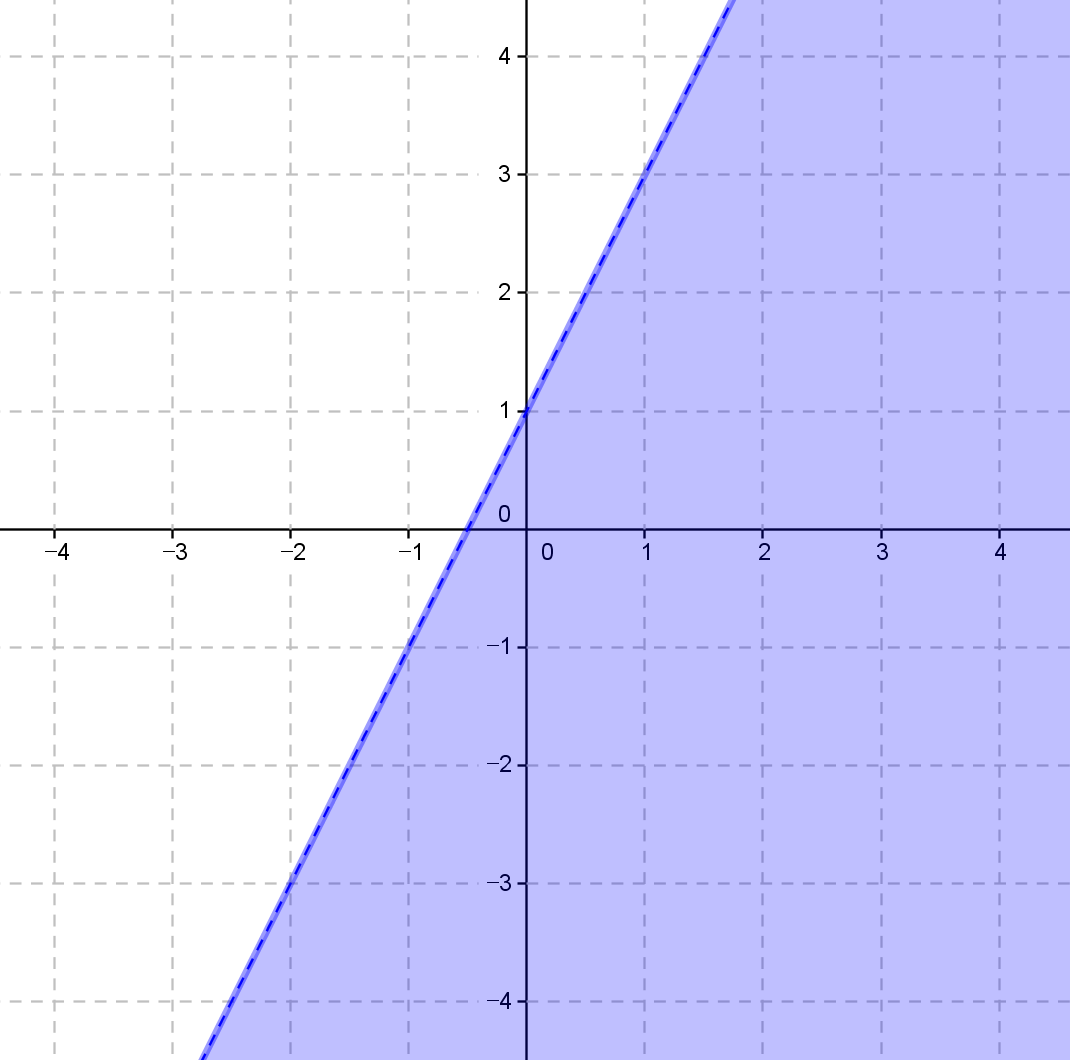
\includegraphics[width=\textwidth]{1-1}\subcaption{}
        \end{subfigure}\quad
        \begin{subfigure}[b]{0.18\textwidth}
                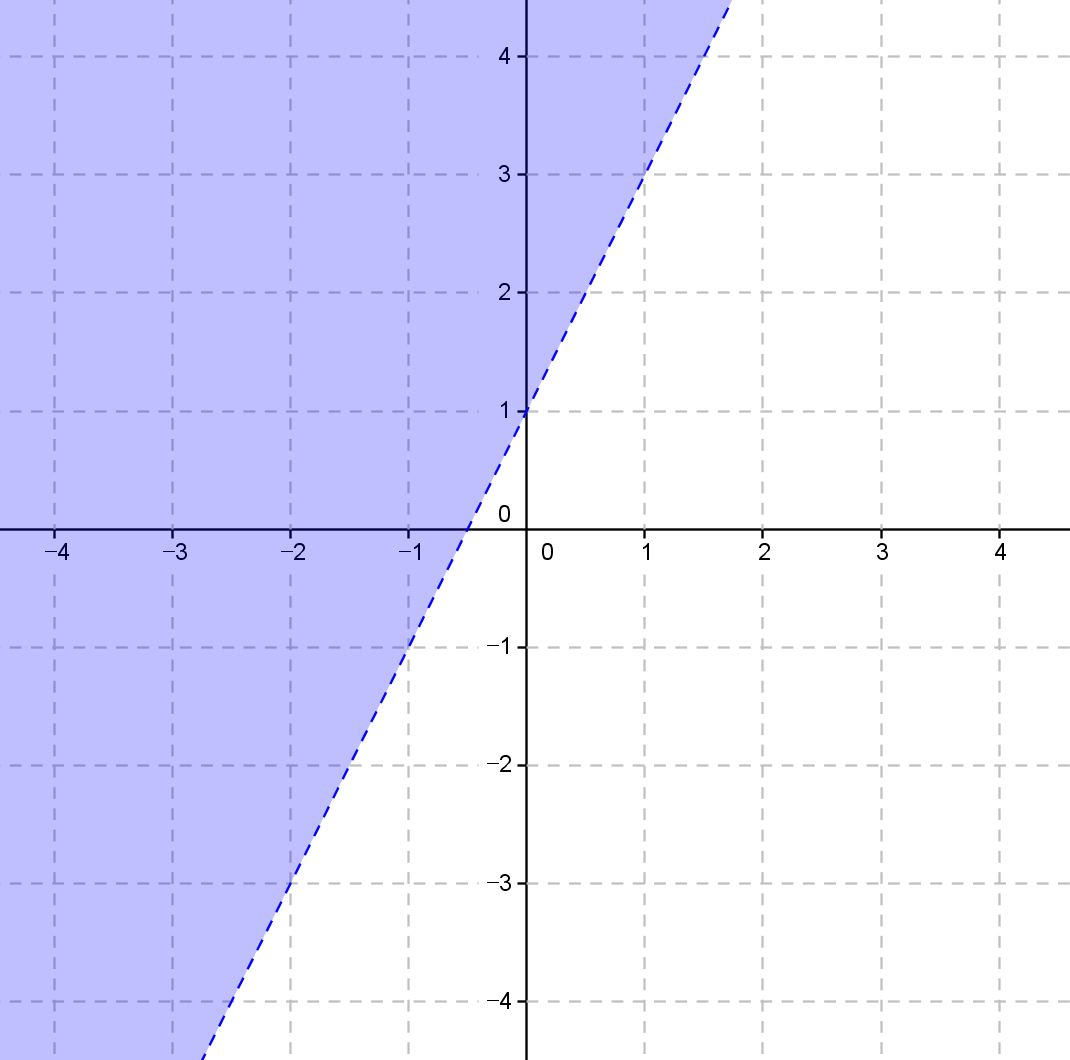
\includegraphics[width=\textwidth]{1-2}\subcaption{}
        \end{subfigure}\par				
        \begin{subfigure}[b]{0.18\textwidth}
                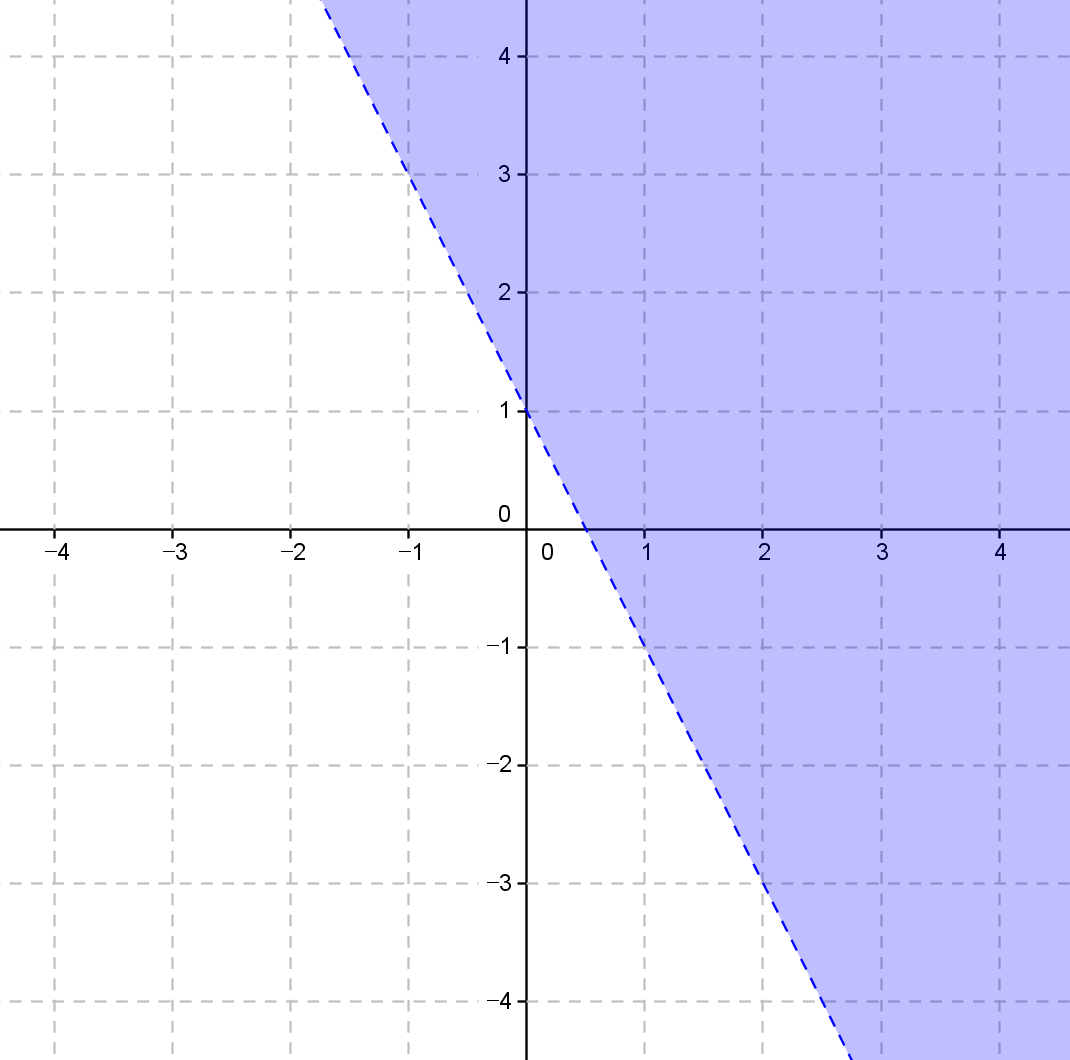
\includegraphics[width=\textwidth]{1-3}\subcaption{}
        \end{subfigure}\quad
        \begin{subfigure}[b]{0.18\textwidth}
                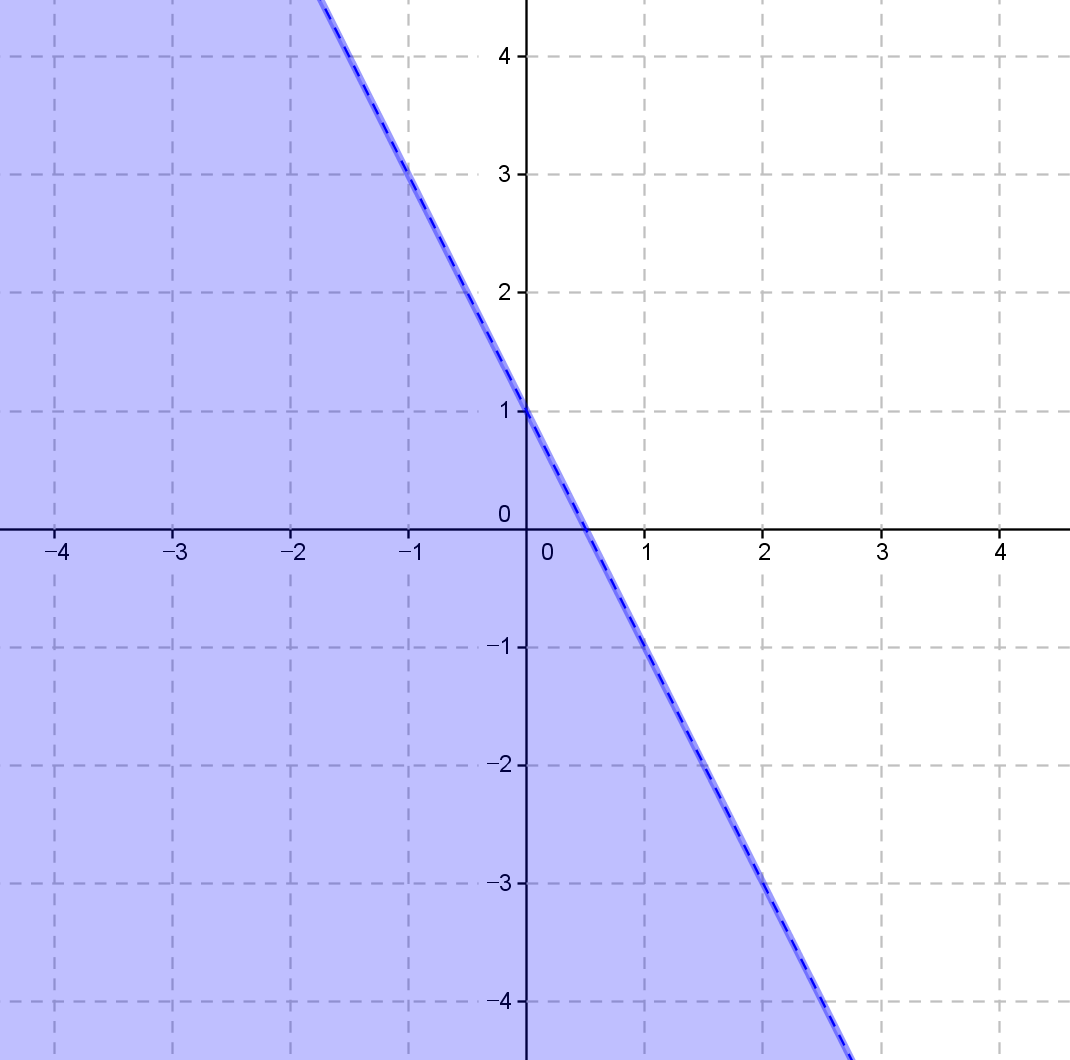
\includegraphics[width=\textwidth]{1-4}\subcaption{}
        \end{subfigure}
\end{figure}

\howo{}
다음 부등식의 영역을 좌표 평면 위에 나타내어라.
\[2x+3y+6>0\]

\begin{figure}[h!]
        \centering
        \begin{subfigure}[b]{0.18\textwidth}
                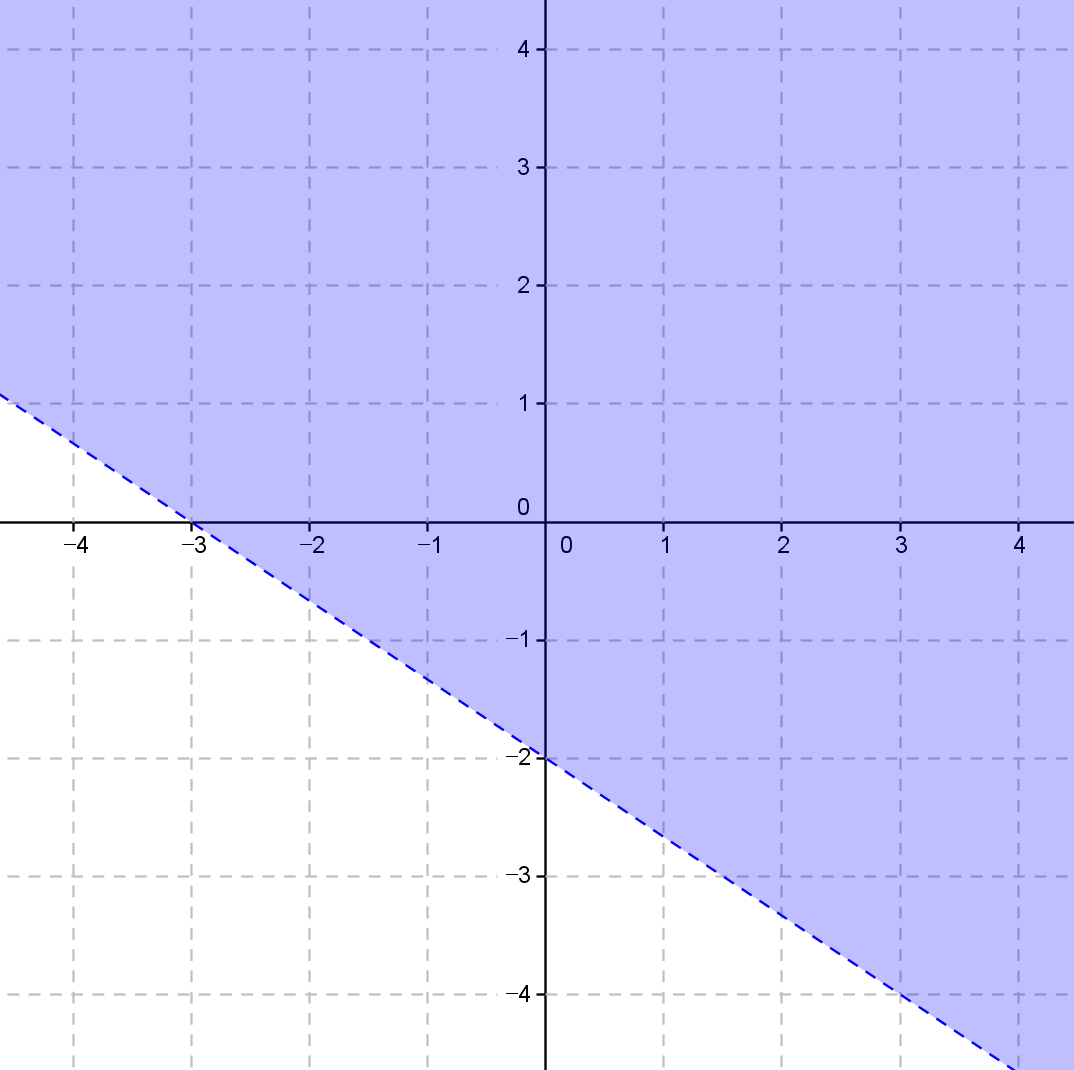
\includegraphics[width=\textwidth]{2-1}\subcaption{}
        \end{subfigure}\quad
        \begin{subfigure}[b]{0.18\textwidth}
                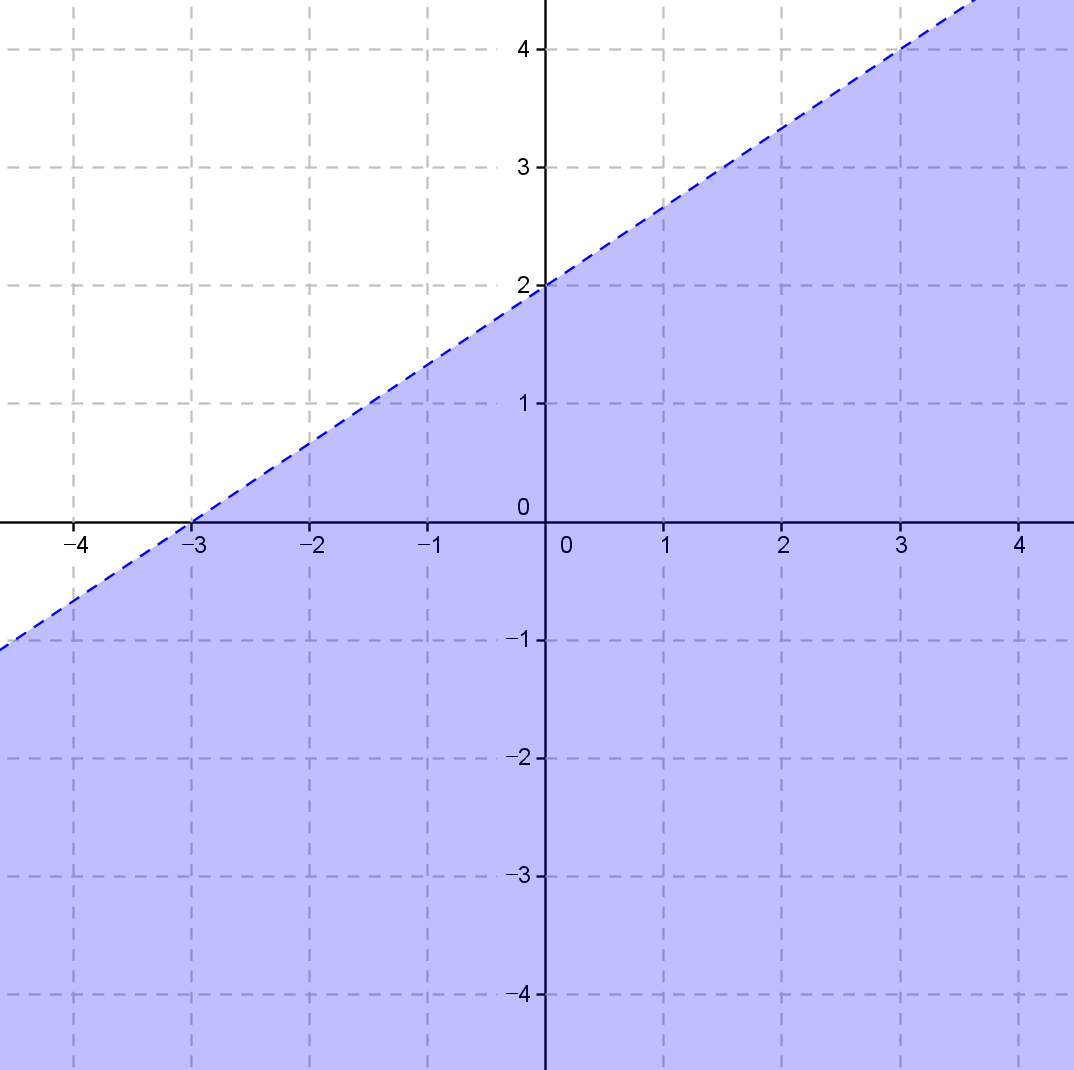
\includegraphics[width=\textwidth]{2-2}\subcaption{}
        \end{subfigure}\par				
        \begin{subfigure}[b]{0.18\textwidth}
                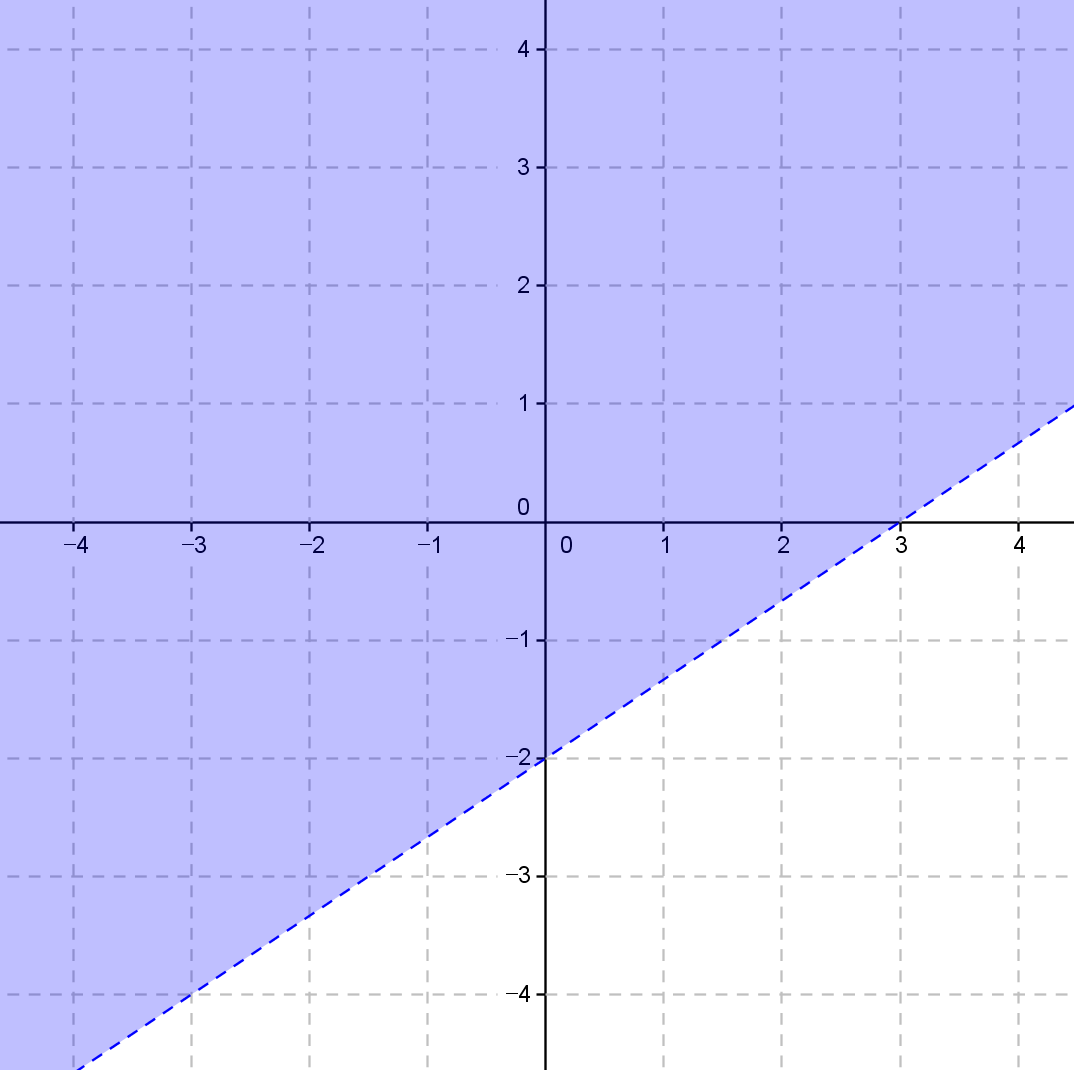
\includegraphics[width=\textwidth]{2-3}\subcaption{}
        \end{subfigure}\quad
        \begin{subfigure}[b]{0.18\textwidth}
                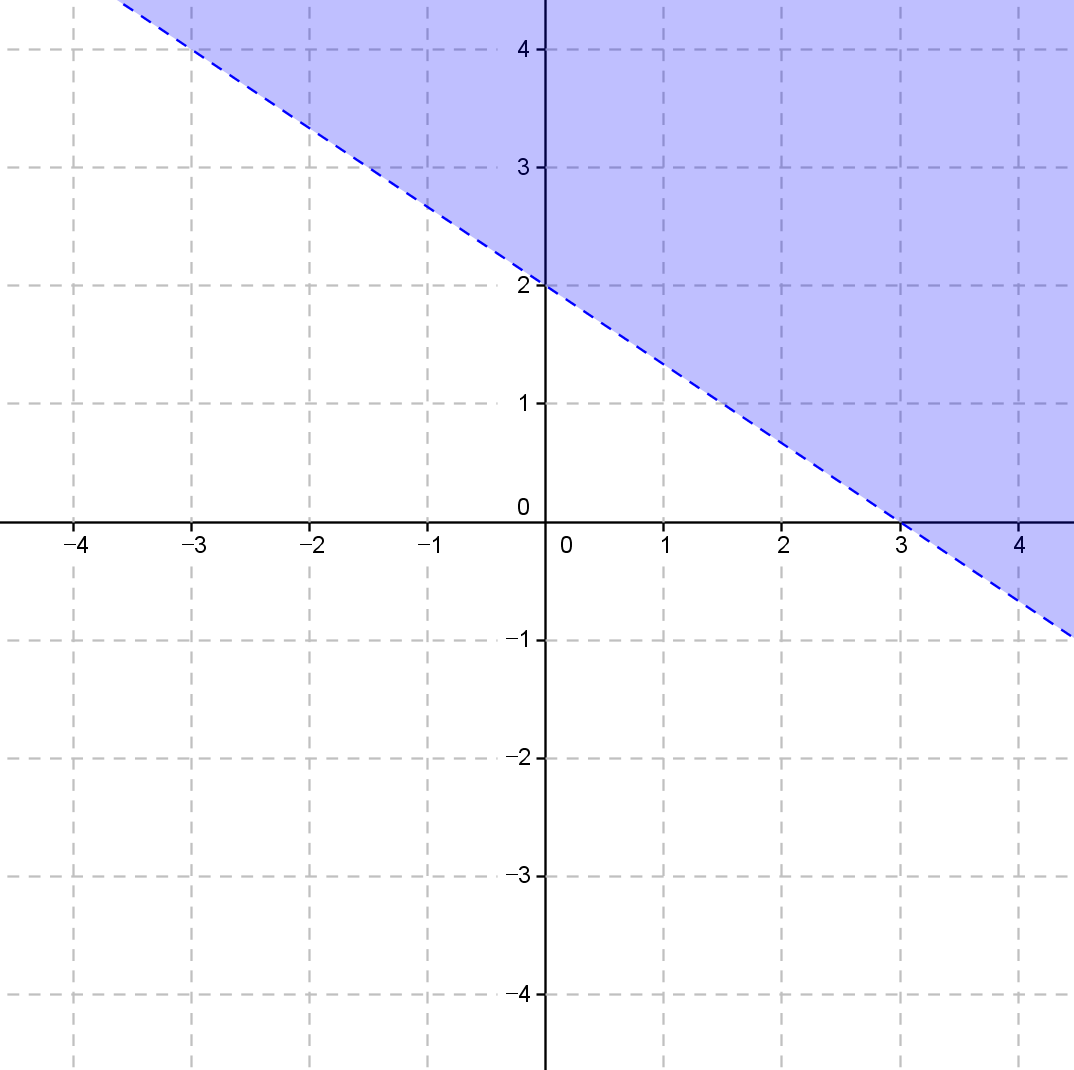
\includegraphics[width=\textwidth]{2-4}\subcaption{}
        \end{subfigure}
\end{figure}

\howo{}
다음 부등식의 영역을 좌표 평면 위에 나타내어라.
\[x^2+y^2-4x<0\]


\begin{figure}[h!]
        \centering
        \begin{subfigure}[b]{0.18\textwidth}
                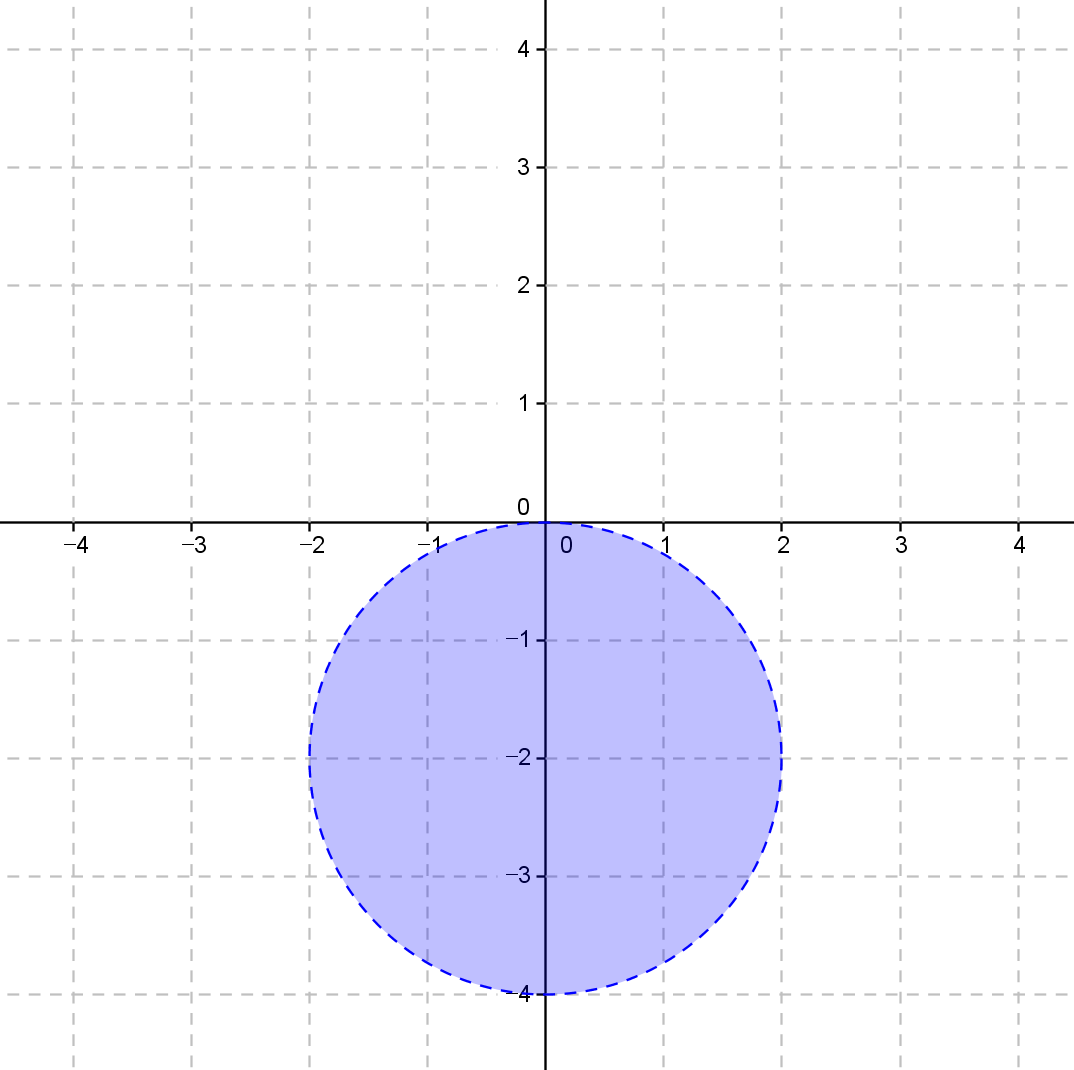
\includegraphics[width=\textwidth]{3-1}\subcaption{}
        \end{subfigure}\quad
        \begin{subfigure}[b]{0.18\textwidth}
                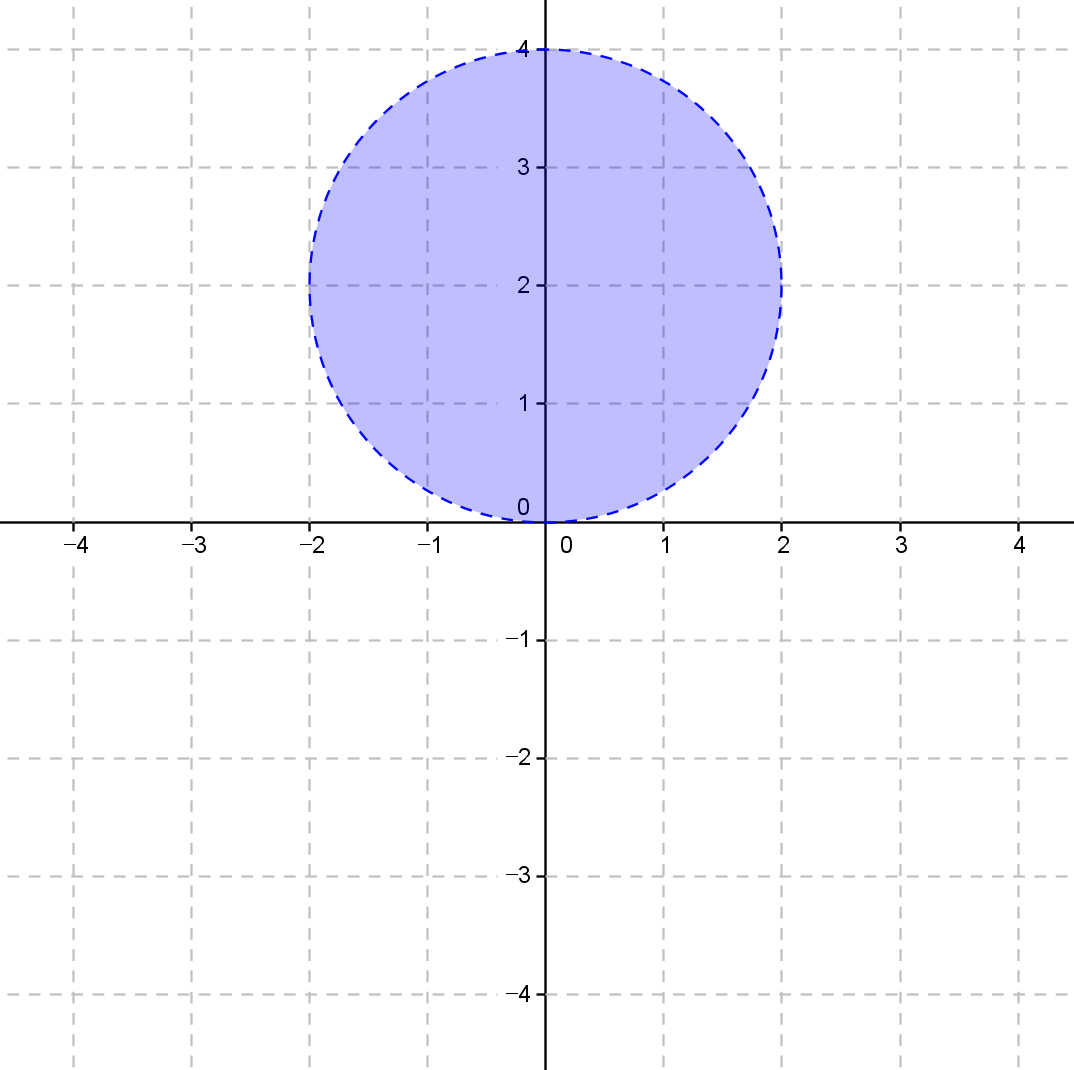
\includegraphics[width=\textwidth]{3-2}\subcaption{}
        \end{subfigure}\par				
        \begin{subfigure}[b]{0.18\textwidth}
                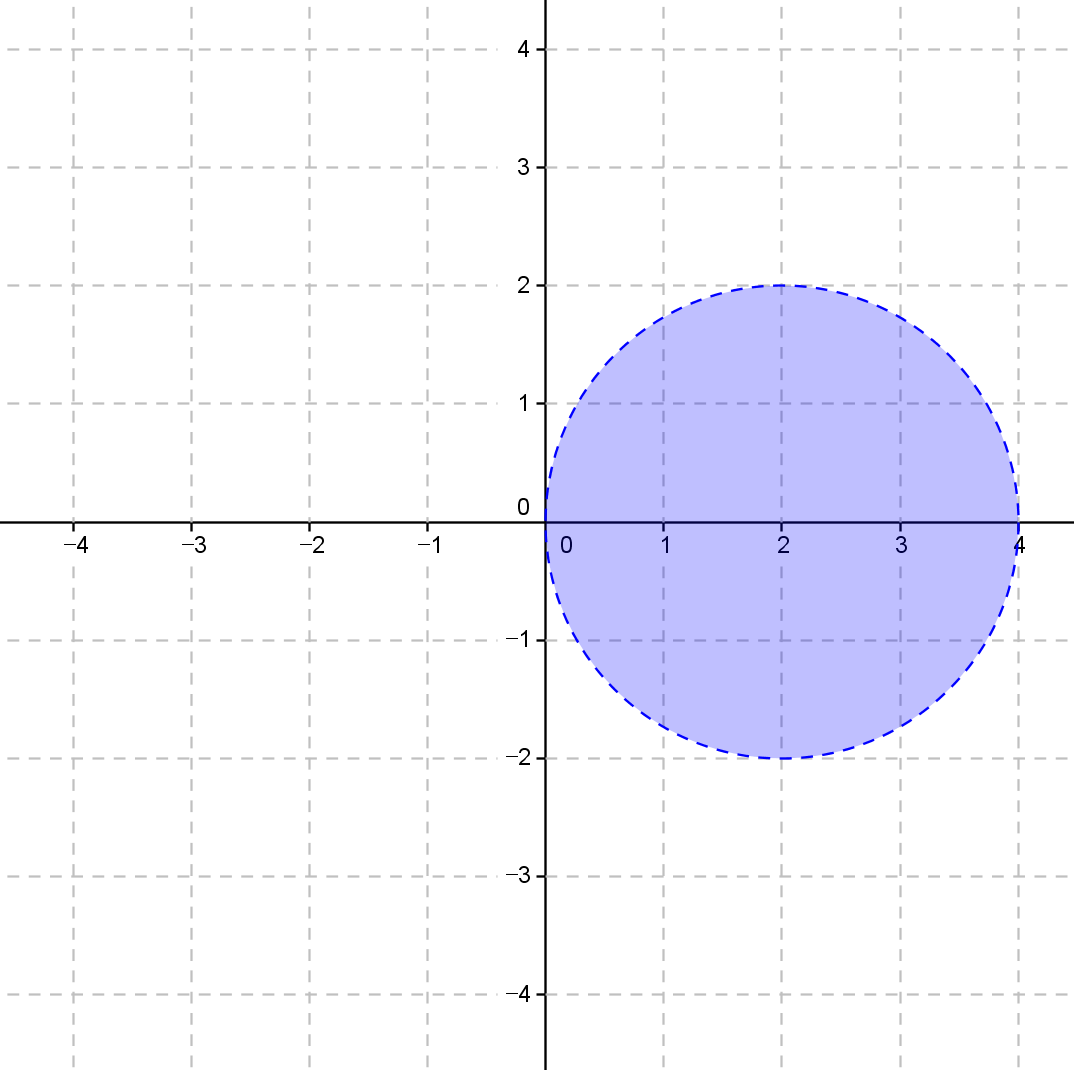
\includegraphics[width=\textwidth]{3-3}\subcaption{}
        \end{subfigure}\quad
        \begin{subfigure}[b]{0.18\textwidth}
                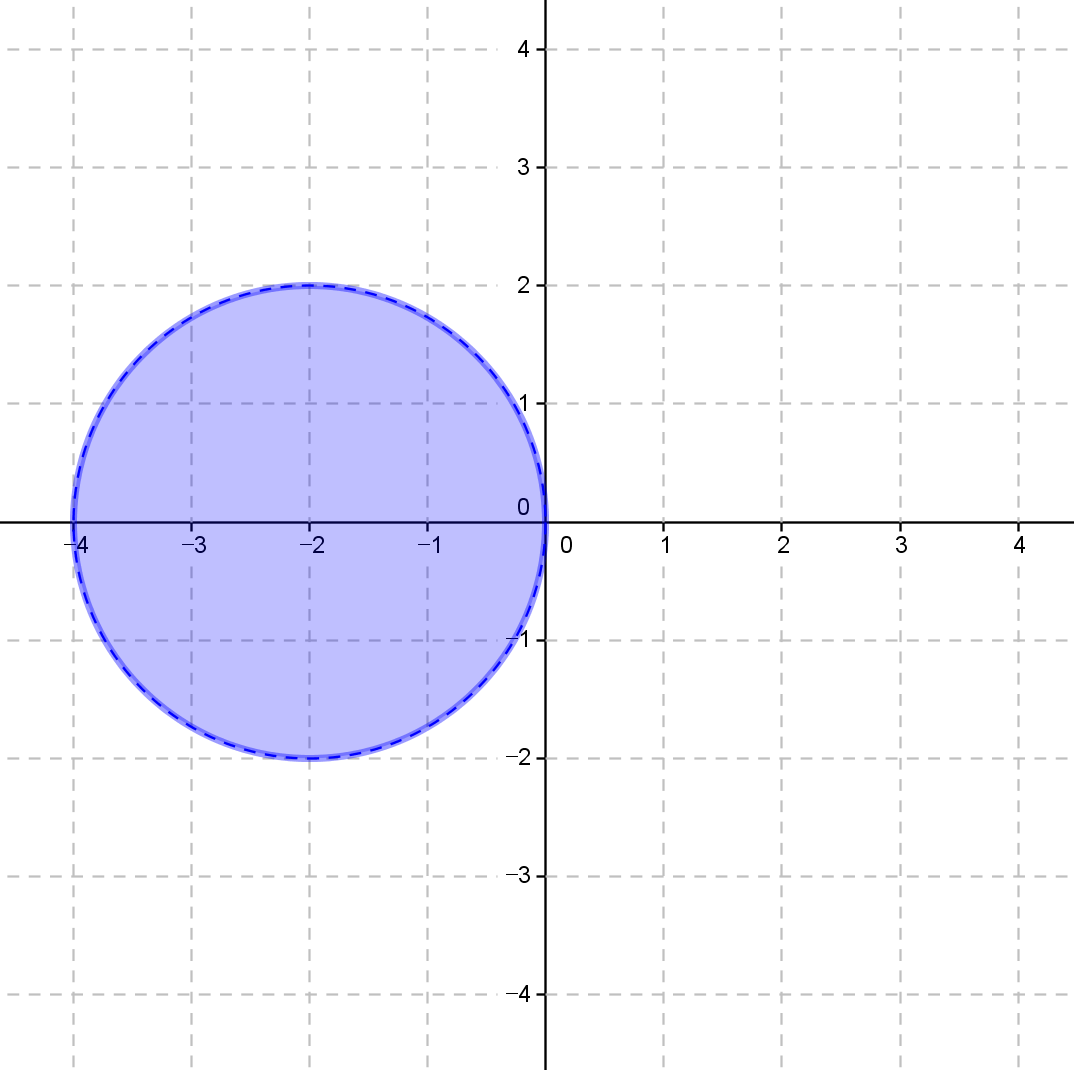
\includegraphics[width=\textwidth]{3-4}\subcaption{}
        \end{subfigure}
\end{figure}


\howo{}
다음 부등식의 영역을 좌표 평면 위에 나타내어라.
\[y>x^2+2x+3\]


\begin{figure}[h!]
        \centering
        \begin{subfigure}[b]{0.18\textwidth}
                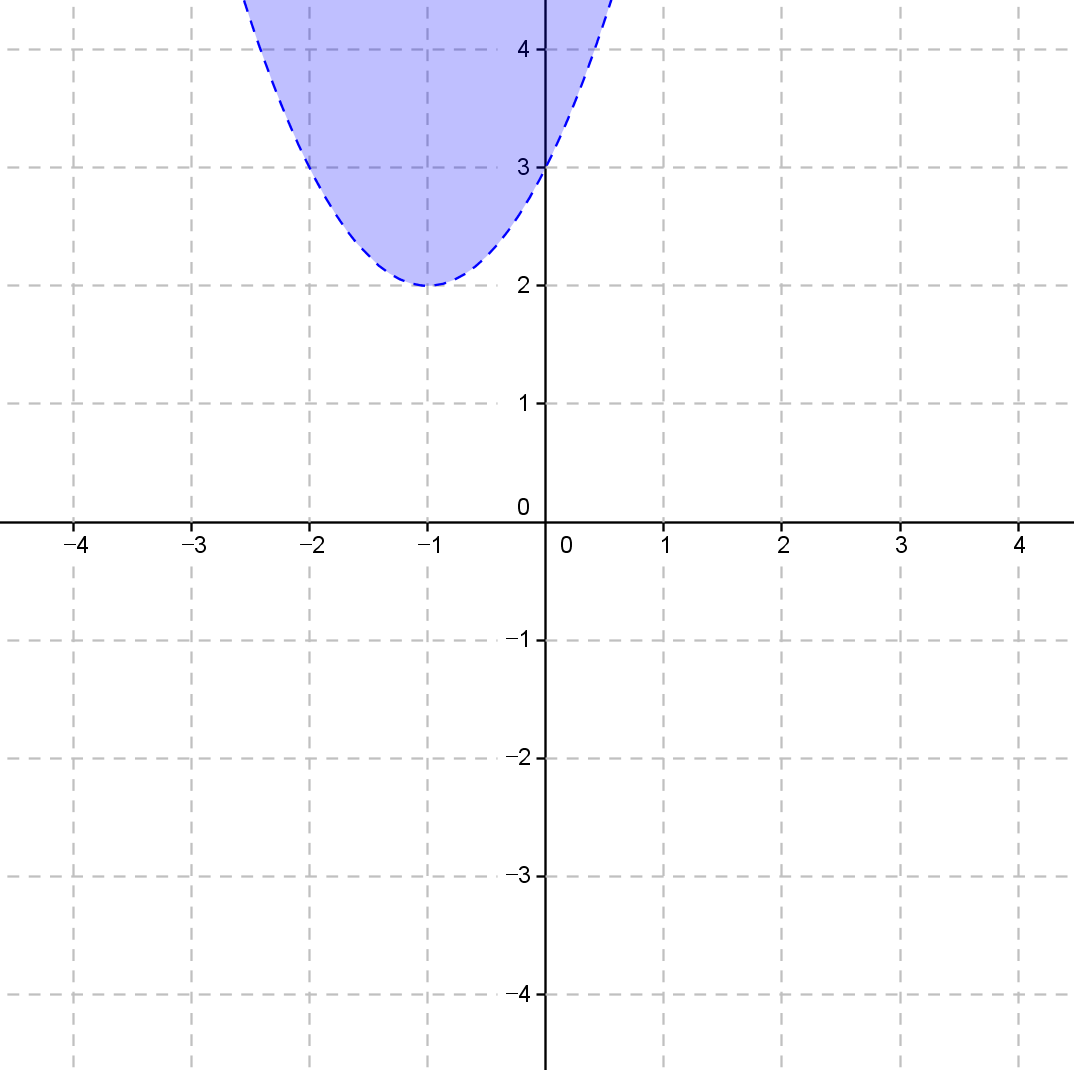
\includegraphics[width=\textwidth]{4-1}\subcaption{}
        \end{subfigure}\quad
        \begin{subfigure}[b]{0.18\textwidth}
                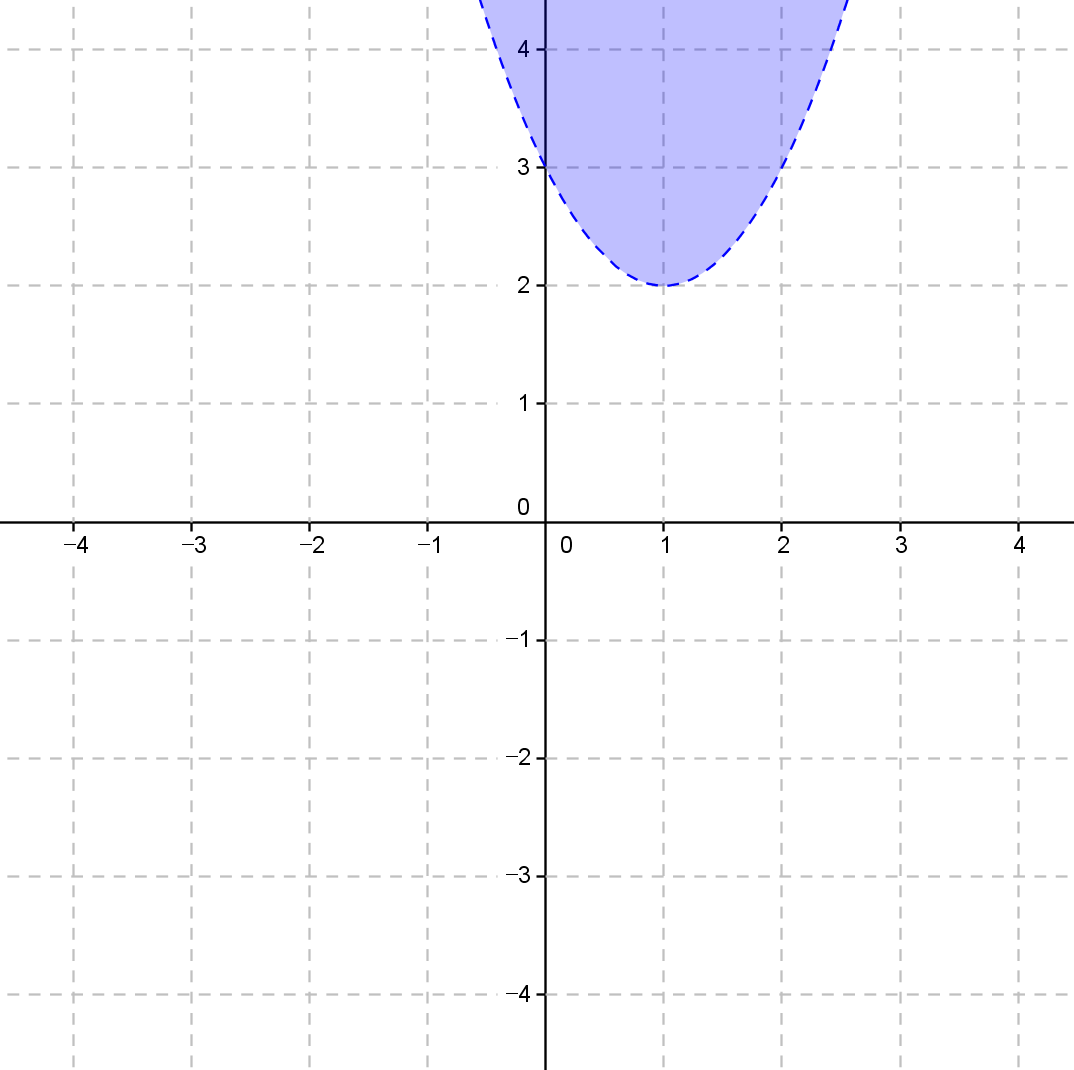
\includegraphics[width=\textwidth]{4-2}\subcaption{}
        \end{subfigure}\par				
        \begin{subfigure}[b]{0.18\textwidth}
                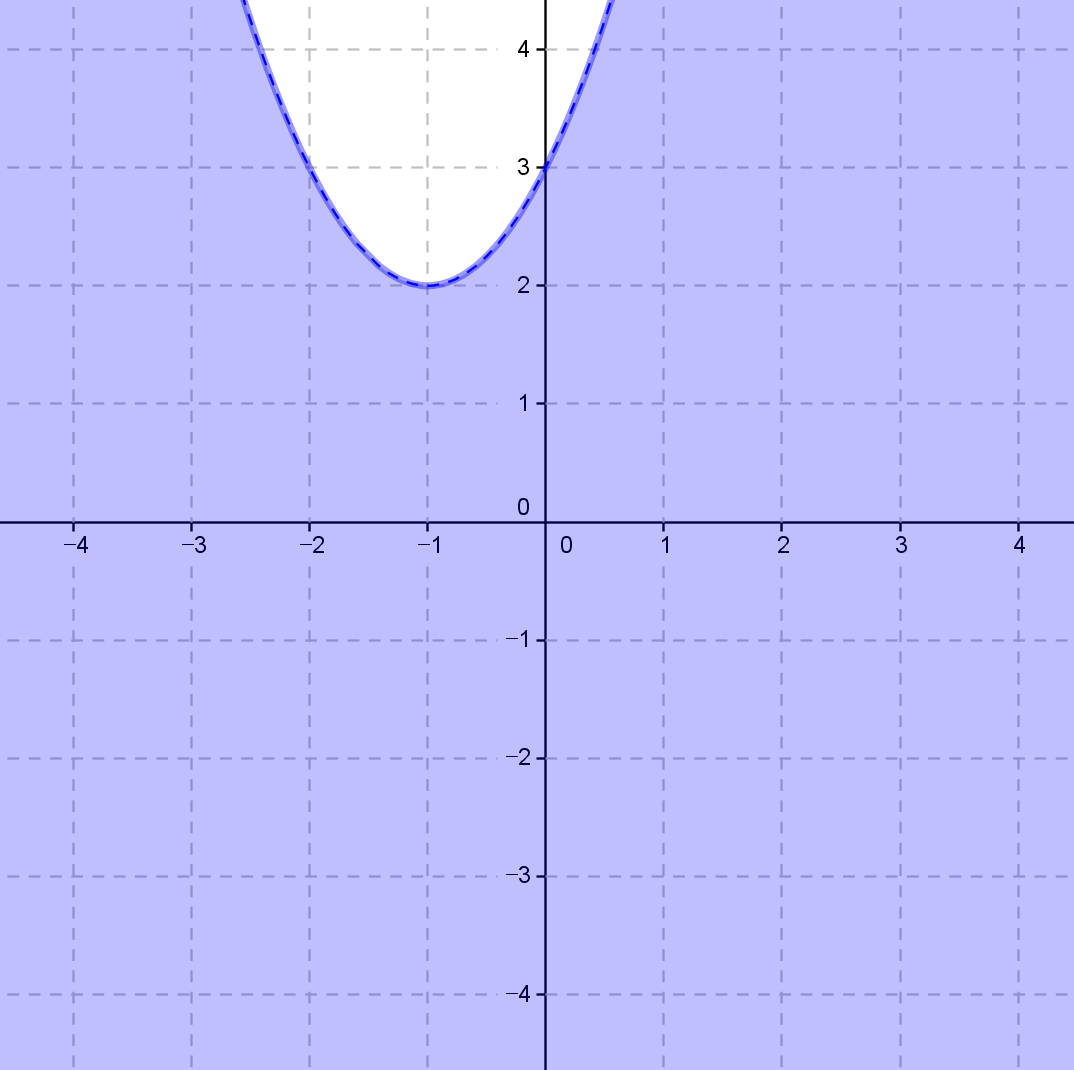
\includegraphics[width=\textwidth]{4-3}\subcaption{}
        \end{subfigure}\quad
        \begin{subfigure}[b]{0.18\textwidth}
                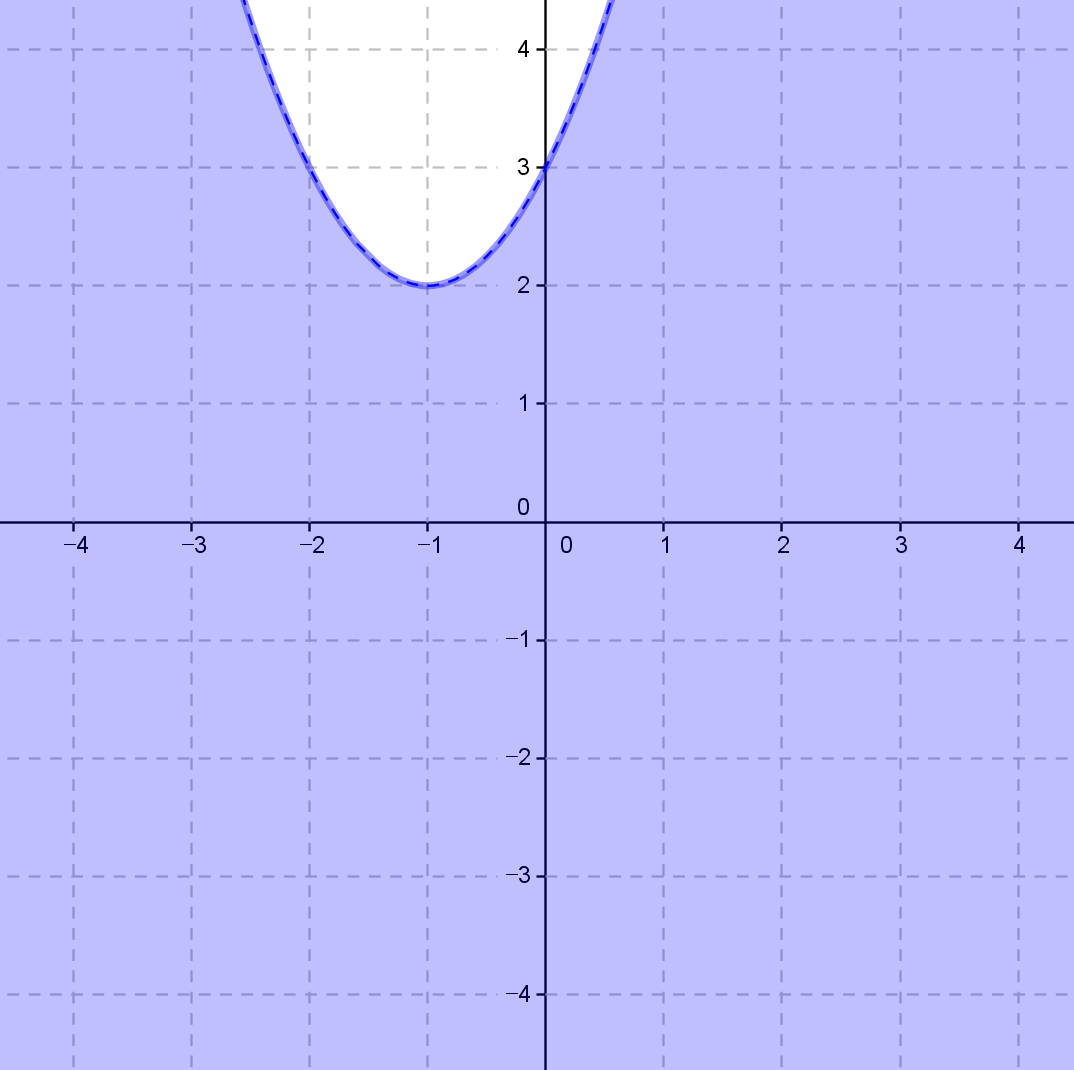
\includegraphics[width=\textwidth]{4-4}\subcaption{}
        \end{subfigure}
\end{figure}

\newpage

\howo{}
다음 그림에서 색칠된 영역을 부등식으로 나타내어라.
\begin{figure}[h!]
\centering
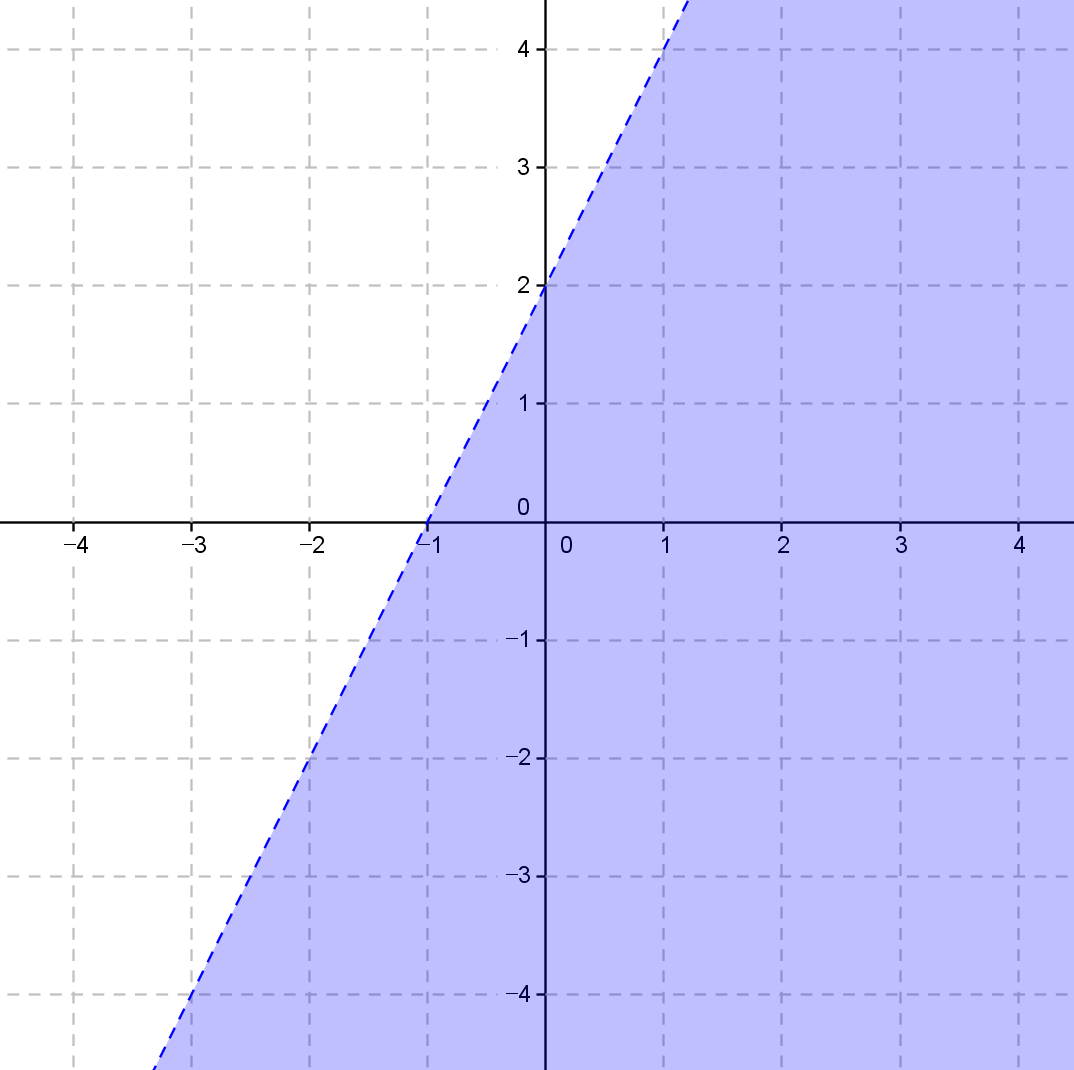
\includegraphics[width=0.4\textwidth]{5-1}
\end{figure}

%
\howo{}
다음 연립부등식의 영역을 좌표 평면 위에 나타내어라.\\
\[
\begin{cases}
y\le x+2\\
x^2+y^2<9
\end{cases}
\]

\begin{figure}[h!]
        \centering
        \begin{subfigure}[b]{0.18\textwidth}
                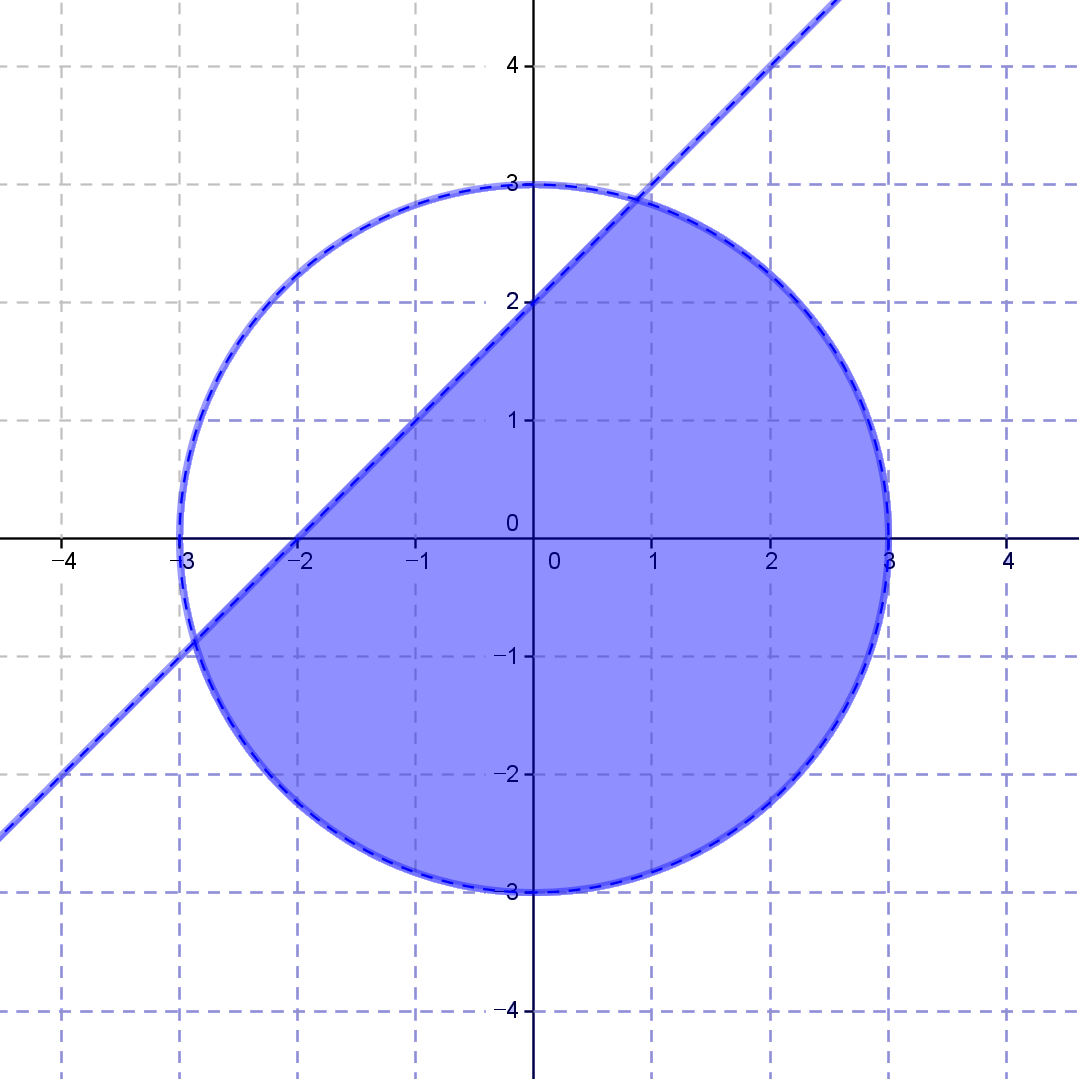
\includegraphics[width=\textwidth]{6-1}\subcaption{}
        \end{subfigure}\quad
        \begin{subfigure}[b]{0.18\textwidth}
                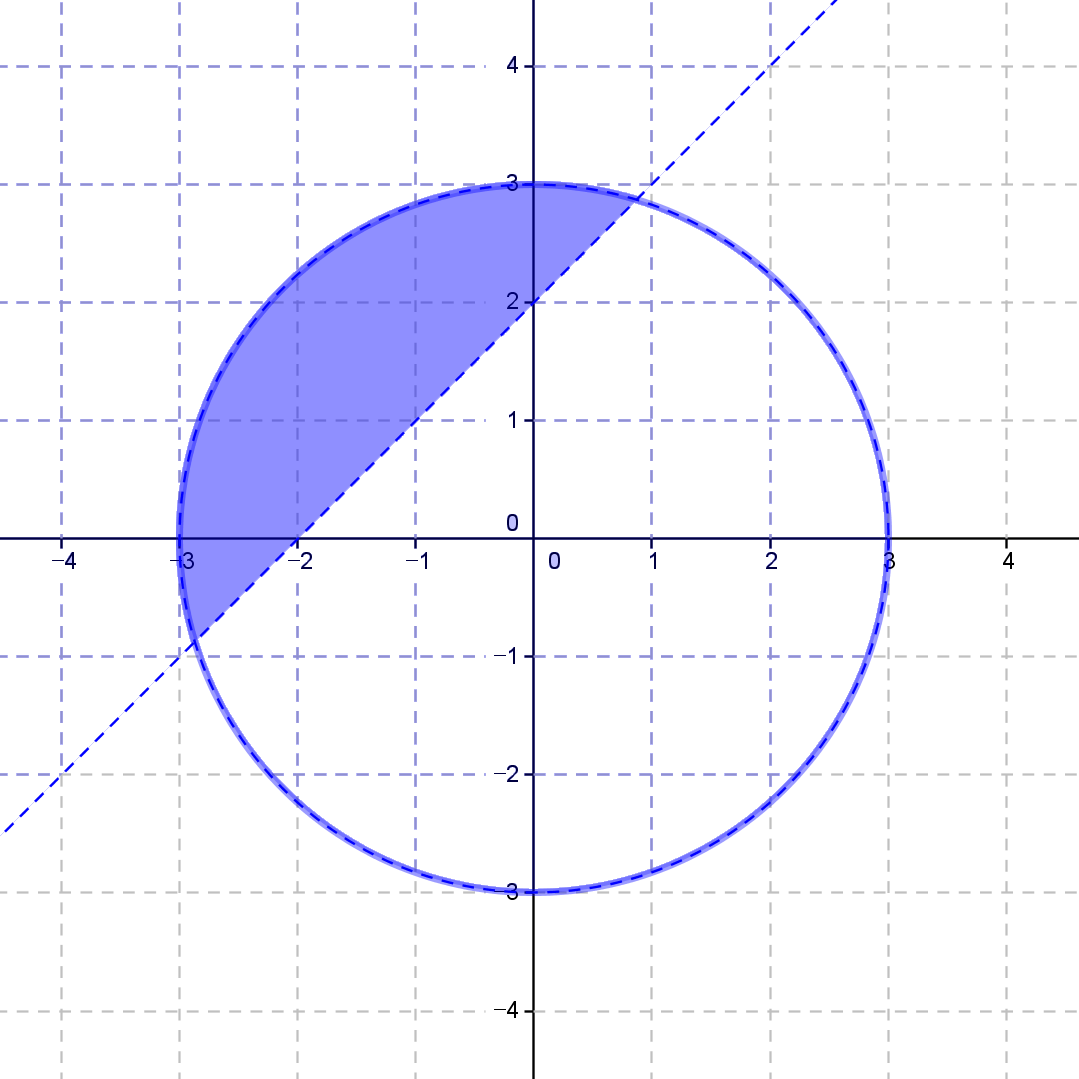
\includegraphics[width=\textwidth]{6-2}\subcaption{}
        \end{subfigure}\par				
        \begin{subfigure}[b]{0.18\textwidth}
                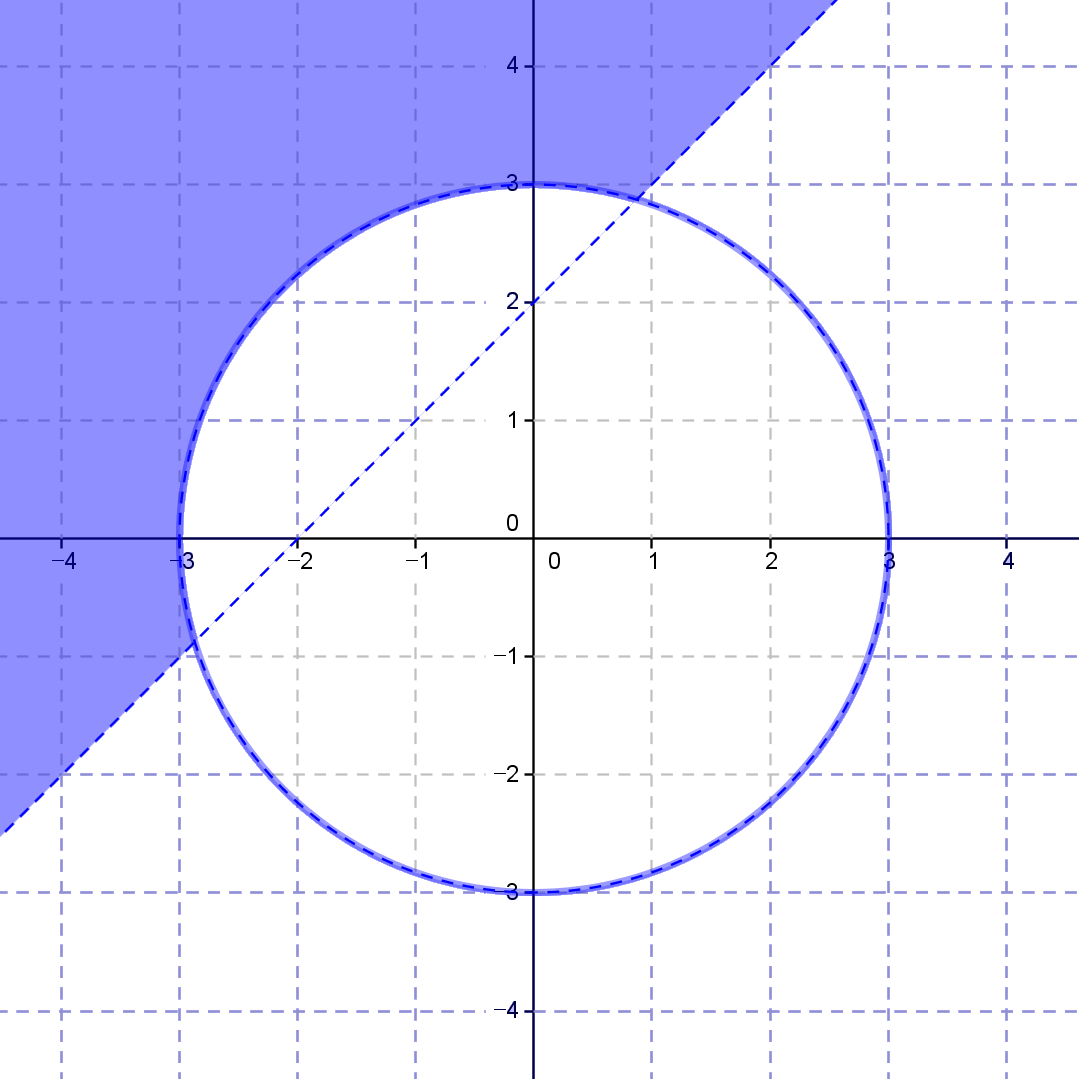
\includegraphics[width=\textwidth]{6-3}\subcaption{}
        \end{subfigure}\quad
        \begin{subfigure}[b]{0.18\textwidth}
                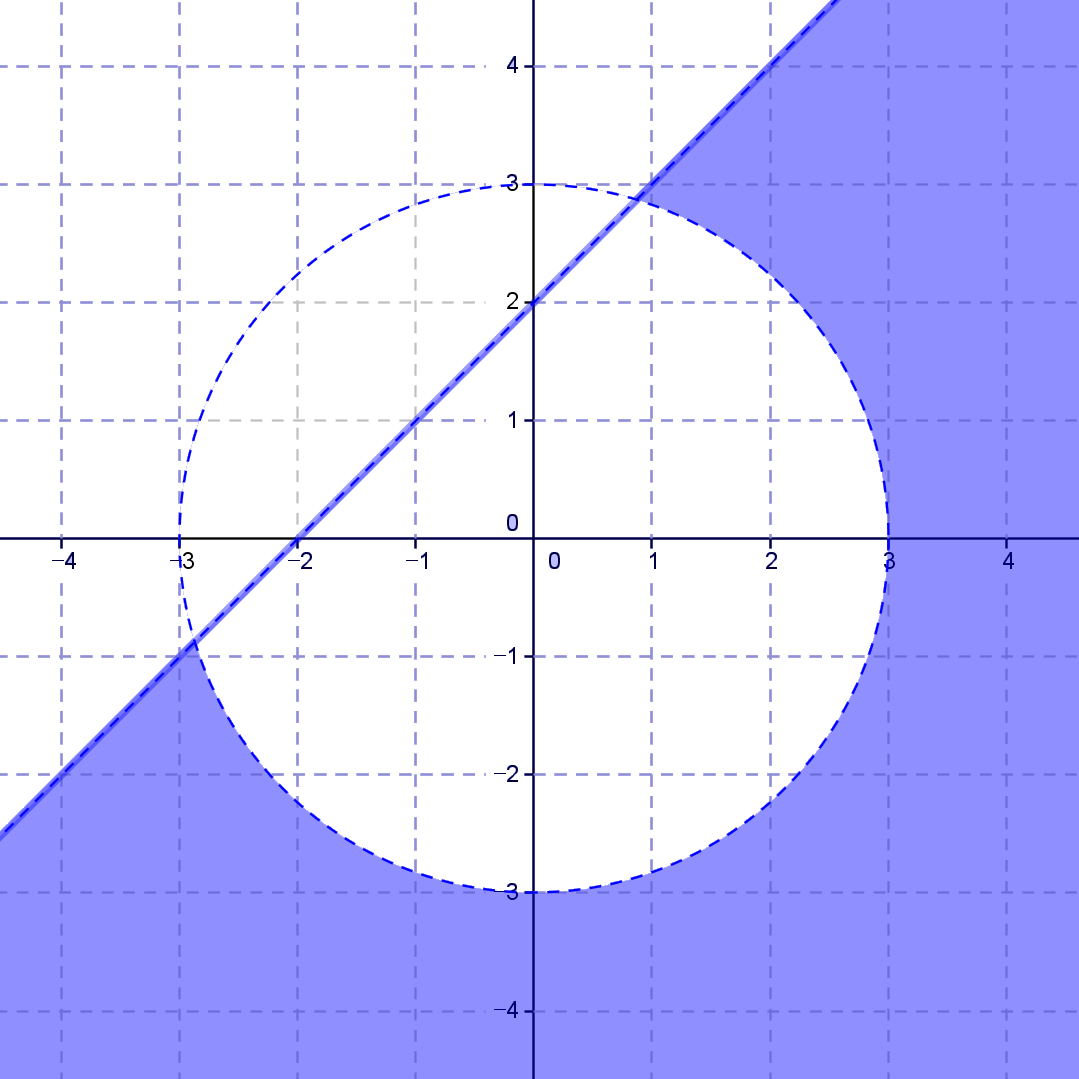
\includegraphics[width=\textwidth]{6-4}\subcaption{}
        \end{subfigure}
\end{figure}

\newpage
%
\howo{}
다음 부등식의 영역을 좌표 평면 위에 나타내어라.\\
\[(x - 2y + 4) (x + y)  >  0\]

\begin{figure}[h!]
        \centering
        \begin{subfigure}[b]{0.18\textwidth}
                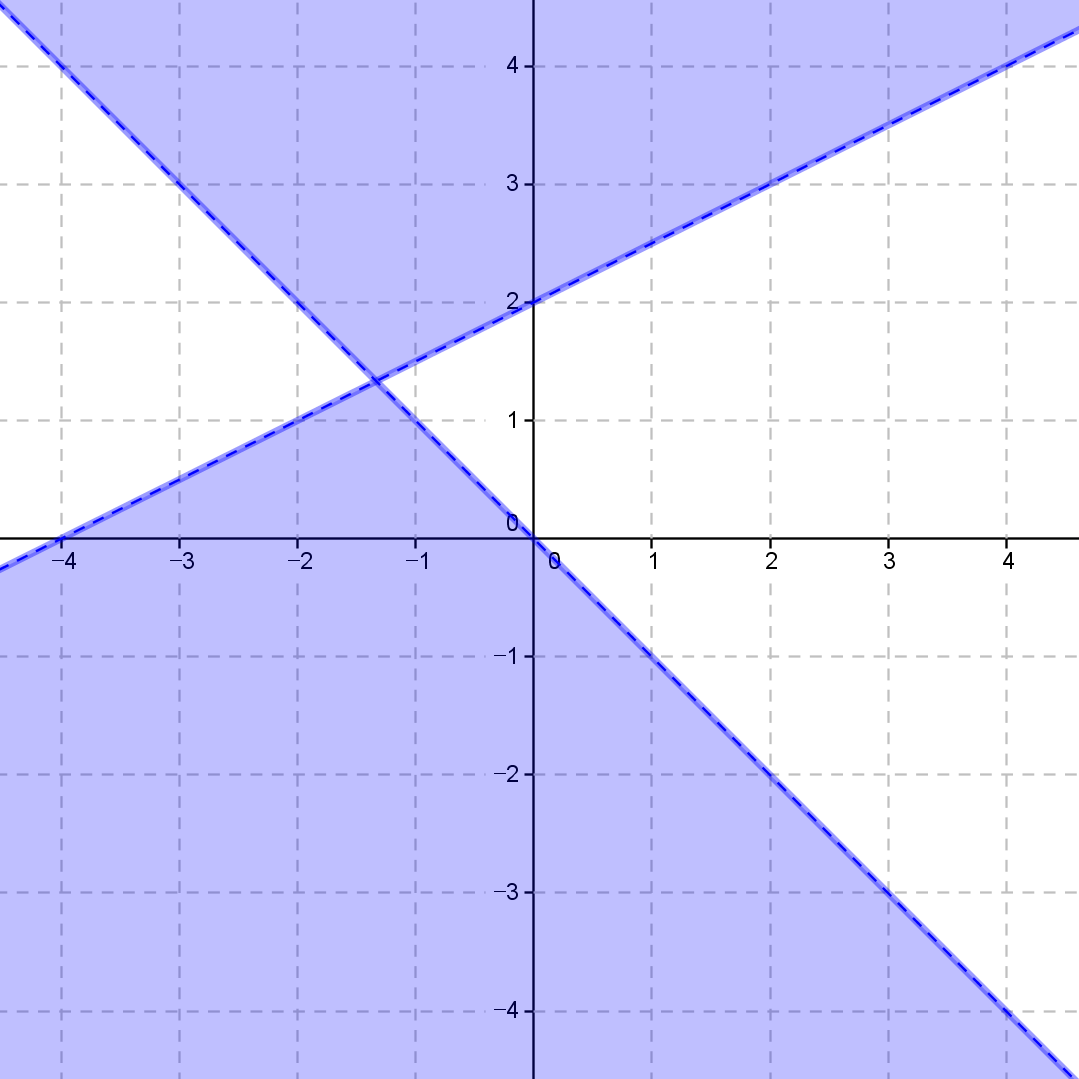
\includegraphics[width=\textwidth]{7-1}\subcaption{}
        \end{subfigure}\quad
        \begin{subfigure}[b]{0.18\textwidth}
                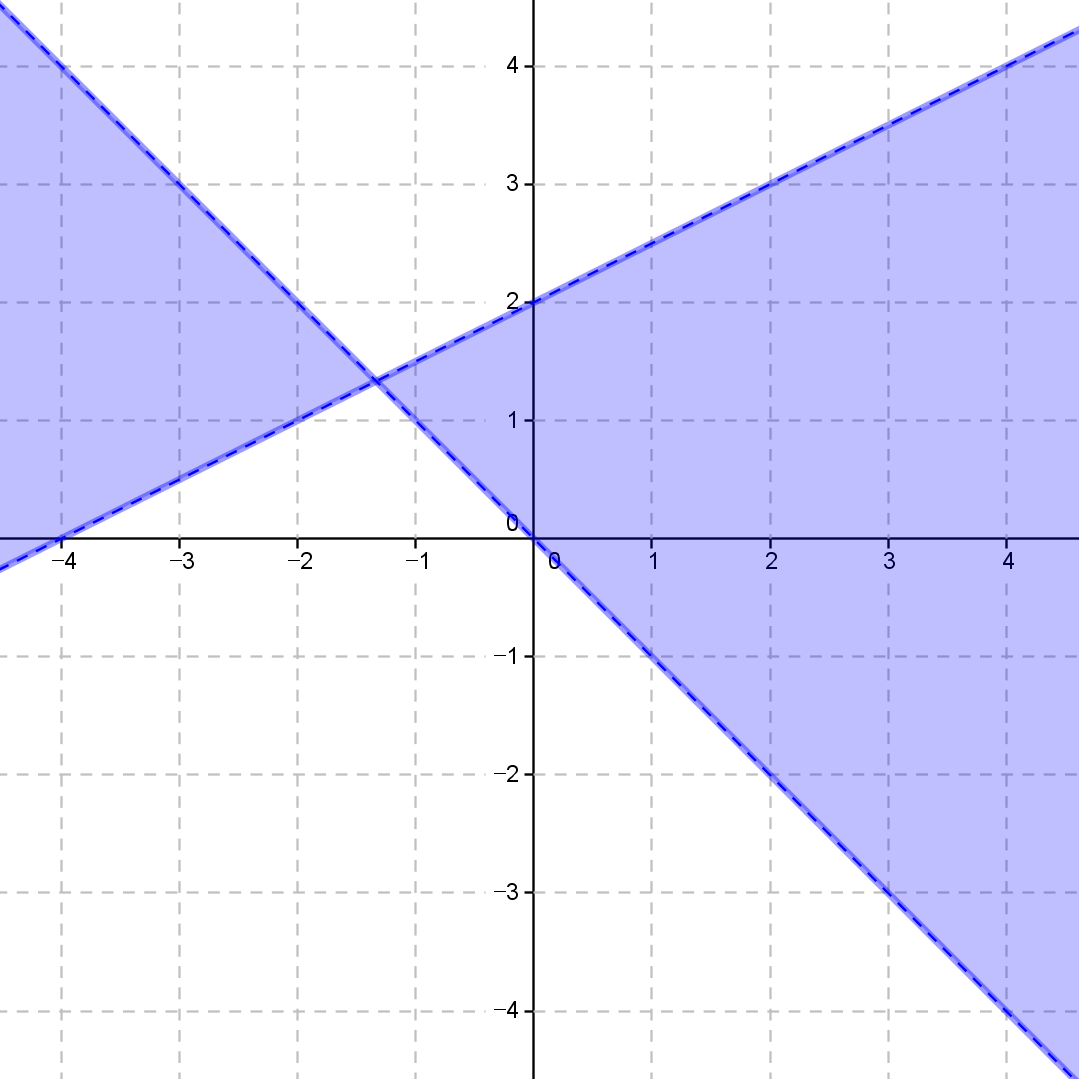
\includegraphics[width=\textwidth]{7-2}\subcaption{}
        \end{subfigure}\par				
        \begin{subfigure}[b]{0.18\textwidth}
                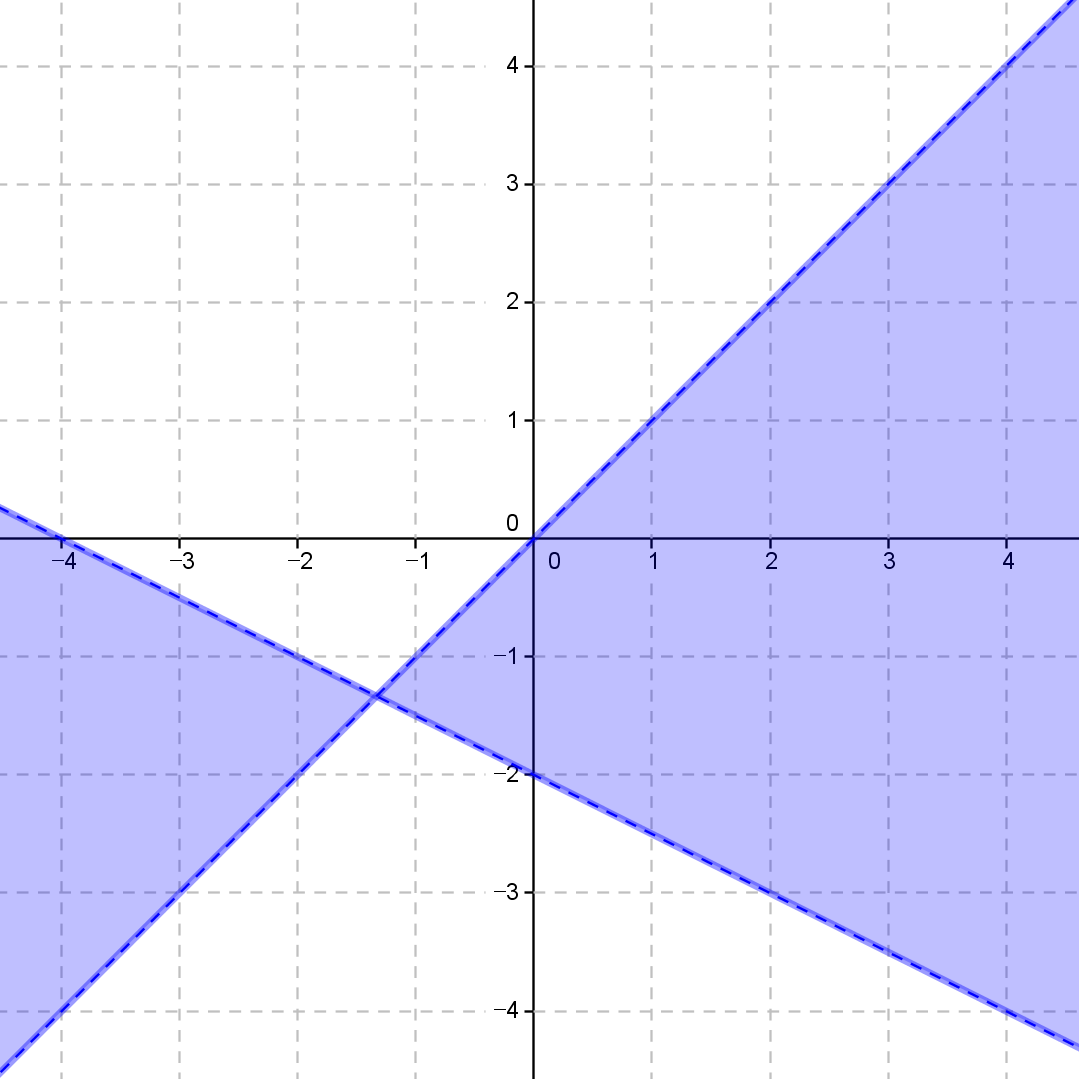
\includegraphics[width=\textwidth]{7-3}\subcaption{}
        \end{subfigure}\quad
        \begin{subfigure}[b]{0.18\textwidth}
                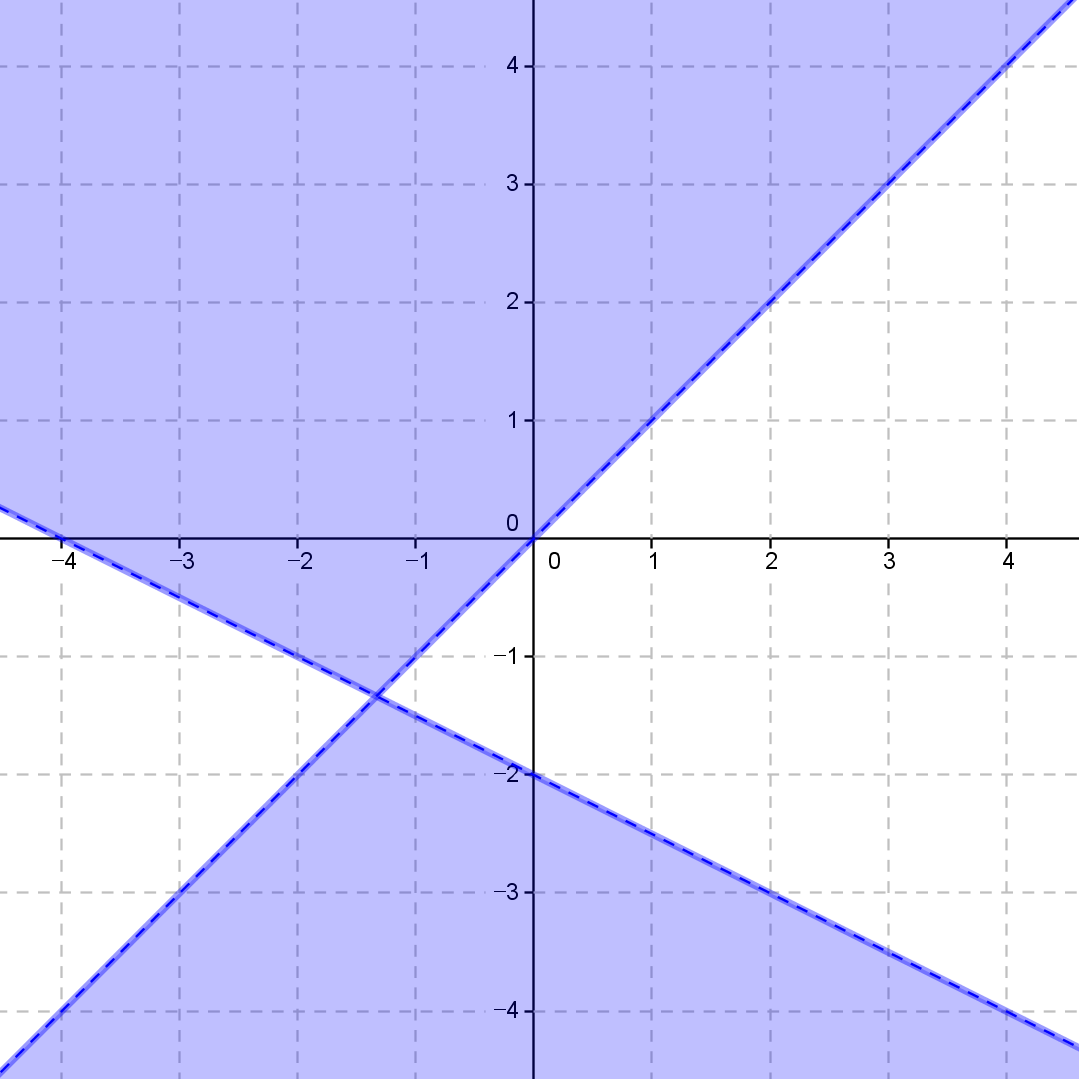
\includegraphics[width=\textwidth]{7-4}\subcaption{}
        \end{subfigure}
\end{figure}

%
\howo{}
다음 부등식의 영역을 좌표 평면 위에 나타내어라.\\
\[(x - 2y + 4) (x + y)  >  0\]

\begin{figure}[h!]
        \centering
        \begin{subfigure}[b]{0.18\textwidth}
                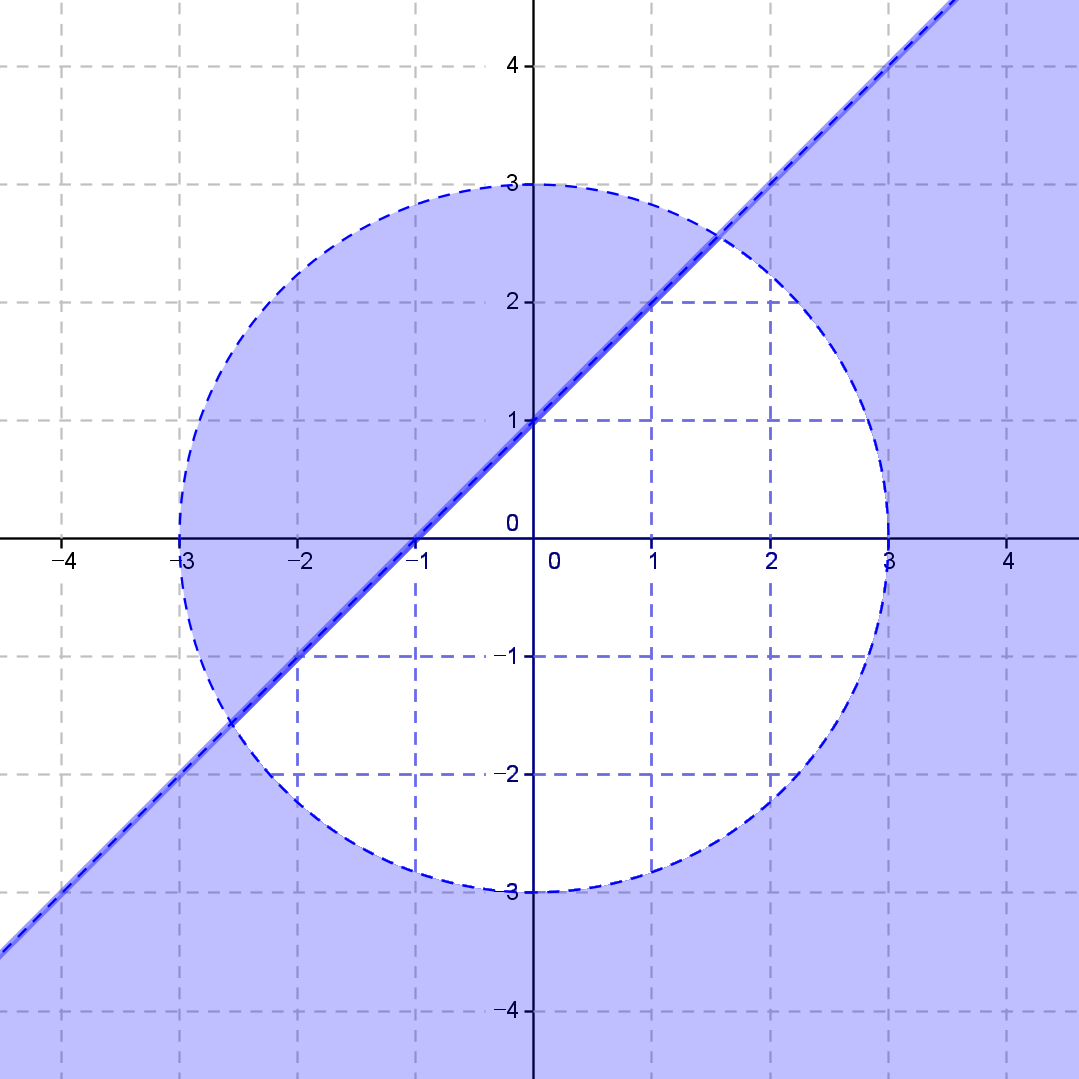
\includegraphics[width=\textwidth]{8-1}\subcaption{}
        \end{subfigure}\quad
        \begin{subfigure}[b]{0.18\textwidth}
                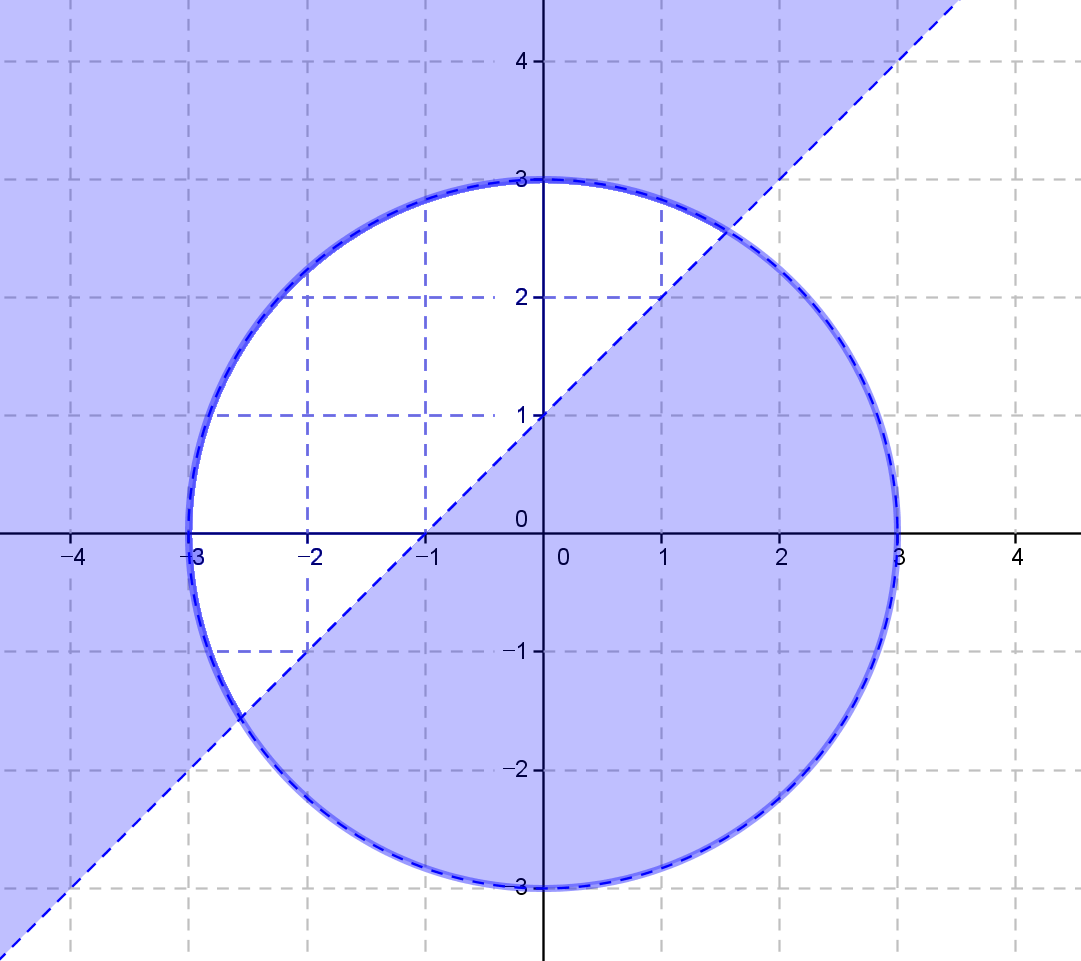
\includegraphics[width=\textwidth]{8-2}\subcaption{}
        \end{subfigure}\par				
        \begin{subfigure}[b]{0.18\textwidth}
                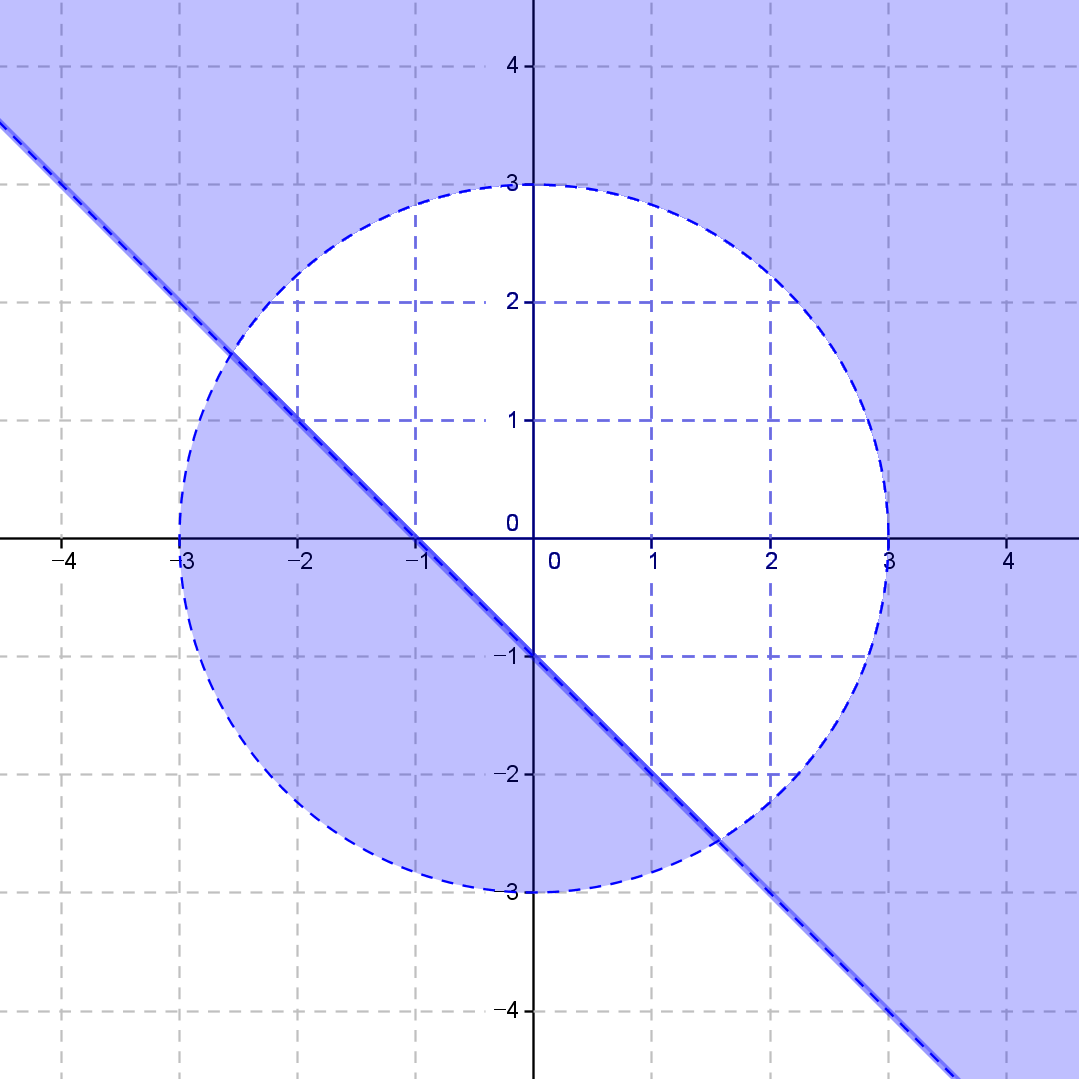
\includegraphics[width=\textwidth]{8-3}\subcaption{}
        \end{subfigure}\quad
        \begin{subfigure}[b]{0.18\textwidth}
                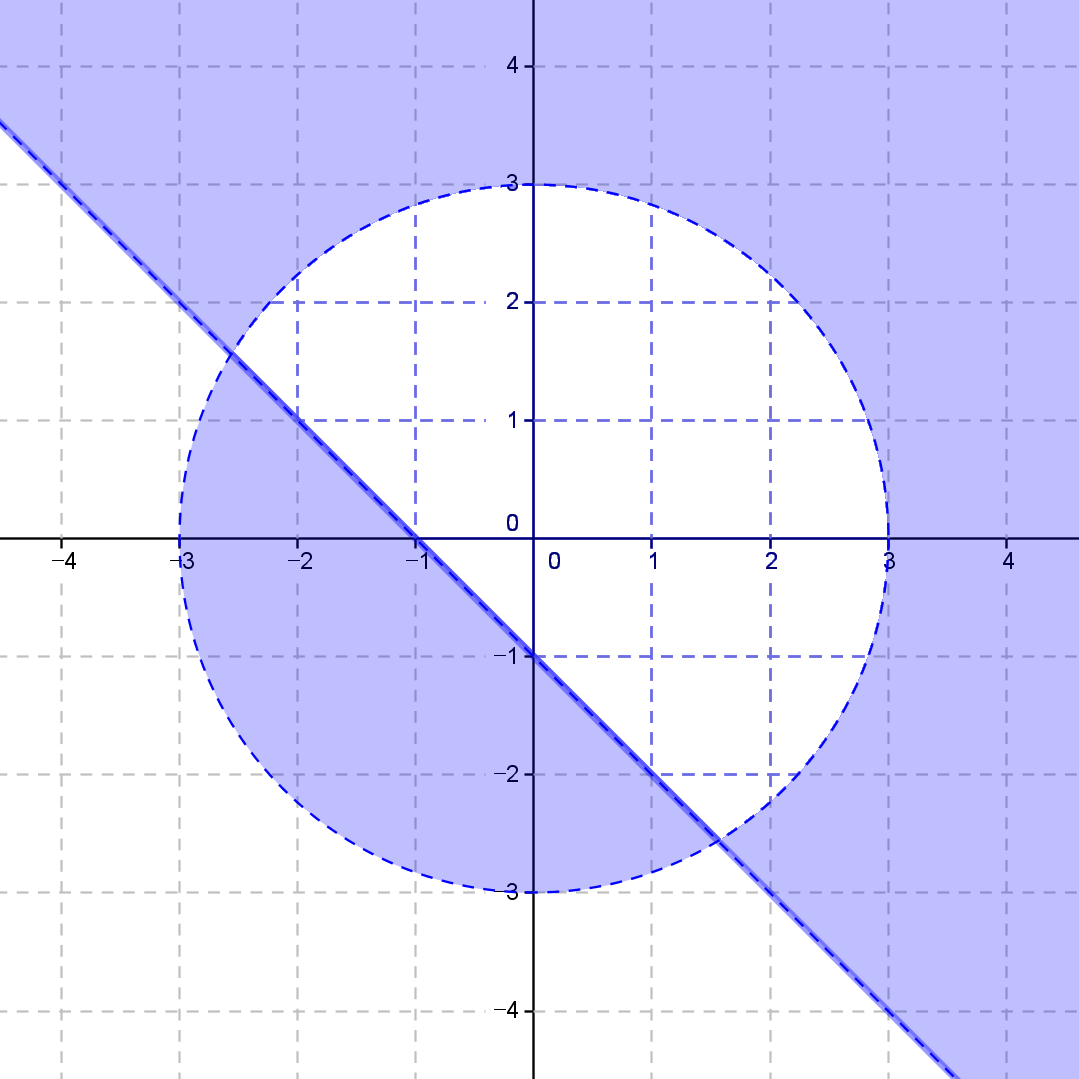
\includegraphics[width=\textwidth]{8-4}\subcaption{}
        \end{subfigure}
\end{figure}

\newpage

%
\howo{}
연립부등식 \(x\ge0\), \(y\ge0\), \(x+2y\le 6\), \(2x+y\le6\)에서 \(x+y\)의 최댓값을 구하여라.


%
\howo{}
연립부등식 \(x\ge0\), \(y\ge0\), \(x+3y\le 7\), \(2x+y\le5\)에서 \(x+y\)의 최댓값을 구하여라.

%
\howo{}
연립부등식 \(x\ge0\), \(y\ge0\), \(2x+3y\le 10\), \(2x+y\le6\)에서 \(x+y\)의 최댓값을 구하여라.
\end{document}